% !TEX options=--shell-escape

\documentclass{article}
\usepackage{tikz,polyglossia,amsthm,amsmath,cancel,pgfplots,animate,multirow,unicode-math,adjustbox,booktabs,array,pst-solides3d,pst-all,pst-3dplot,mathtools,multicol,graphicx,float,svg}

\title{Молекулярно-кинетическая теория \\ \large Дополнительные главы физики}
\date{Апрель 2022}
\author{Иван Мачуговский}

\usetikzlibrary{automata,positioning,calc,decorations.pathmorphing,patterns,external}
% \tikzexternalize[prefix=external/]

\newcommand{\definition}[2]{\begin{samepage} \textbf{#1} -- #2. \end{samepage} \par}
\newcommand{\namedequation}[2]{\begin{samepage} \textbf{#1}: $\displaystyle#2$. \end{samepage} \par}
\newcommand{\namedlaw}[2]{\begin{samepage} \textbf{#1}: \begin{center}\fbox{\begin{minipage}{0.8\textwidth}#2\end{minipage}}\end{center} \end{samepage} \par}
\newcommand{\namedmultline}[2]{\textbf{#1}: \begin{multline*}#2\end{multline*}\par}
\newcommand{\namednewline}[2]{\textbf{#1}: \par $\displaystyle#2$.\par}
\newcommand{\const}{\mathrm{const}}
\renewcommand{\d}{\mathop{}\!\mathrm{d}}
\newcommand{\abs}[1]{\lvert#1\rvert}

\setlength{\parindent}{0pt}
\setlength{\parskip}{5pt}
\setmainfont{CMU Serif}
\widowpenalties 1 10000
\raggedbottom

\begin{document}
	\maketitle

	Молекулярно-кинетическая теория исследует строение веществ, в основном газов, их свойства, агрегатные состояния и т.п., опираясь на следующие постулаты, многократно доказанные опытом:

	\begin{section}{Постулаты МКТ}
		\begin{enumerate}
			\item Все тела состоят из \textbf{частиц}: молекул для сложных веществ, атомов для более простых, в некоторых случаях--ионов;

			\item Частицы находятся в постоянном хаотическом движении, то есть каждая отдельная частица движется в случайном направлении, и в среднем в каждом направлении движется одинаковое число частиц;

			\item Частицы взаимодействуют друг с другом исключительно путем абсолютно упругих столкновений. Это означает, частицы располагаются настолько далеко друг от друга, что кулоновское взаимодействие между ними пренебрежимо мало.
		\end{enumerate}
	\end{section}


	\begin{section}{Введение в молекулярную физику}
		Химические свойства атома зависят только от заряда его ядра, а не от массы, поэтому существуют разные "виды" атомов одного элемента, отличающиеся количеством нейтронов в ядре.

		\definition{Изотопы}{атомы, имеющие одинаковый заряд и потому одинаково ведущие себя в химических реакциях и занимающие одну и ту же клетку таблицы Менделеева, но имеющие разную массу. Например: протий $\prescript{1}{1}{H}$, дейтерий $D = \prescript{2}{1}{H}$ и тритий $T = \prescript{3}{1}{H}$ являются изотопами водорода $\prescript{}{1}{H}$}

		Хотя протоны в ядрах атома отталкиваются электростатически, по всей видимости, что-то их заставляет не удаляться друг от друга. Это -- сильное взаимодейстие, проявляющееся, вообще говоря, на еще более низком уровне, чем нуклоны, но имеющее такой побочный эффект:

		\definition{Сильное взаимодействие}{взаимодействие, отвечающее за связь между протонам и электронами в ядрах атомов. Действует на расстояниях порядка размера протона. Это не очень корректное определение; истинное сильное взаимодействие проявляется на уровне кварков и описывается КХД, но на уровне нуклонов оно проявляется именно так}
	\end{section}


	\begin{section}{Единицы измерения}
		Поскольку МКТ тесно рассматривает в том числе отдельные частицы и их параметры, которые, будучи выражены в единицах СИ, представляют собой очень малые значения, вводятся микроскопические единицы измерения:

		\definition{1 а.е.м. (атомная единица массы)}{1/12 массы $\prescript{12}{6}{C}$}

		\definition{Относительная атомная масса [а.е.м.]}{отношение массы частицы к 1/12 массе $\prescript{12}{6}{C}$}

		1 а.е.м. очень близка к массе водорода, однако по некоторым причинам измерение отношений массы углерода к массе другого атома проще, чем если бы вместо углерода использовался водород, поэтому экспериментальная шкала использовала углерод.

		\definition{Относительная атомная масса}{отношение массы частицы к 1/12 массе углерода-12 $\prescript{12}{6}{C}$}

		В задачах (в основном химических) часто требуется провести вычисления, опирающиеся не на массы, объемы и другие физические свойства, а на количество взаимодействующих частиц. Количество частиц разных веществ, участвующих в химической реакции, например, должно быть пропорционально стехиометрическим коэффициентам. И если относительное количество частиц в двух веществах еще можно легко измерить, скажем, через массы или объемы, или добавляя к одному веществу другое, пока не прекратится реакция, то задача измерения (а, тем более, точного) количества частиц в килограмме данного вещества химикам долго не поддавалась.

		Было введено понятие количества вещества, которое является макроскопическим выражением для количества частиц и, соответственно, прямо пропорционально ему, но в качестве точки отсчета использует макроскопические свойства. Побочный эффект заключается в том, что в практических задачах количество вещества представляет собой не такое огромное число, как число частиц.

		\definition{Количество вещества $\nu$ [моль]}{физическая величина, характеризующая количество структурных единиц (частиц: атомов, молекул, ионов, электронов) вещества}

		Изначально единица моль вводилась для удобства вычислений как:

		\definition{1 моль}{такое количество вещества, что 1 моль углерода-12 $\prescript{12}{6}{C}$ имеет массу 12 г}

		Для перевода между двумя используется экспериментально измеренная константа:

		\definition{Число Авогадро $N_A$ [моль$^{-1}$]}{количество молекул в 1 моле вещества. В единицах СИ $N_A = 6.02214086 \cdot 10^{23}$ моль}

		Затем моль был отвязан от углерода и зафиксирован как

		\definition{1 моль}{$N_A$ молекул, причем $N_A$ является универсальной константой, а не измеримой величиной}

		\definition{Молярная масса $\mu$ [г/моль]}{отношение массы вещества к его количеству. Для однородных веществ она зависит только от составляющих его атомов и численно равна относительной атомной массе частиц}

		Соответственно,

		\namedequation{Количество вещества $\nu$ [моль]}{\nu = \frac{N}{N_A} = \frac{m}{\mu}}

		Кроме того, важными параметрами являются:

		\namedequation{Плотность вещества $\rho$ [кг/м$^3$]}{\rho = \frac{m}{V}}

		\namedequation{Концентрация частиц $n$ [м$^{-3}$]}{n = \frac{N}{V}}
	\end{section}


	\begin{section}{Агрегатные состояния вещества}
		До перехода к описанию МКТ и выводу различных теорем и утверждений для газов стоит обсудить, что такое газ вообще.

		Вещество в первом приближении может находиться в трех агрегатных состояниях. Твердое тело не деформируется самопроизвольно, его частицы часто образуют решетку. Жидкость деформируется относительно свободно, но все еще занимает постоянный объем. Газ же занимает весь отведенный ему объем.

		Эти качественные различия обусловлены, очевидно, не только различными кинетическими энергиями частиц, составляющих вещество. Газ с замедленными частицами при прочих равных условиях оставался бы таким же газом, только более медленным.

		Помимо внутренней кинетической энергии, газ обладает также потенциальной энергией за счет взаимодействий между самими частицами. Природа этого взаимодействия практически всегда электростатическая.

		Состояние твердого тела, жидкости, газа и вообще любого вещества на микроуровне выражается пространственными положениями каждой из его простейших частиц -- ядер атомов и электронов. Между каждой парой частиц существует электростатическое взаимодействие, в некоторых из пар отвечающих за притяжение, а в некоторых -- за отталкивание. Если просуммировать энергии всех этих взаимодействий, получится некоторое выражение, сложным образом зависящее от положений частиц.

		Где достигается минимум этой суммарной энергии -- сложный вопрос, ответить на который можно разве что экспериментально или симуляцией. Рассмотрим частные случаи.

		Частицы могут быть практически неподвижны. Подобное состояние достигается в твердых телах. С одной стороны, электроны электростатически притягиваются к ядрам атомов и потому стремятся занять место между ними, а с другой, по той же причине ядра атомов стараются занять положение между электронами. Но и находиться слишком близко одноименно заряженные частицы не могут, поэтому существует какое-то предельное расстояние, на котором находятся одноименно заряженные частицы. Таким образом, электроны и ядра атомов находятся более или менее симметрично друг между другом образуют две пересекающиеся симметричные решетки.

		В поляризованных веществах, в которых электрический заряд распеределен по молекуле не равномерно, например в воде, молекулы выстраиваются так, что противополжные концы молекул, которые заряжены зарядами разных знаков, притягиваются сильнее, чем отталкиваются соответственные концы молекул, которые заряжены одинаковыми зарядами. В этом случае за образование структуры отвечает асимметрия заряда.

		Когда частицы имеют некоторую скорость, вещество начинает удаляться от этой идеальной картины. Частицы всегда находятся в движении, поэтому в моменте несимметричность распределения заряда существуют абсолютно всегда. Небольшая асимметрия заряда в одной из частиц приведет к асимметрии в соседних частицах, быстро распространяясь по всему веществу. Это может привести как к постепенному увеличению, так и к постепенному уменьшению объема вещества.

		Когда частицы получают достаточную скорость, чтобы сместиться внутри клетки решетки на заметное расстояние, этот эффект усиливается настолько, что расстояние между частицами волей-неволей увеличивается, что выводит потенциальную энергию из минимума. Это все еще состояние твердого тела.

		Когда частицы получают достаточную скорость, чтобы перескочить в соседнюю клетку решетки, то есть их кинетическая энергия превышает работу, необходимую на переход между барьер между клетками, вещество становится текучим, превращаясь в жидкость.

		Если частицам придать еще большую скорость, так, чтобы их кинетическая энергия превышала потенциальную, т.е. работу, необходимую для выхода из жидкости на бесконечность, частицы получают возможность распространяться по объему пространства, не ограниченному объемом жидкости. Это явление испарения. В этом случае мы говорим о состоянии так называемого насыщенного пара, о котором мы поговорим далее: часть частиц все еще связаны в жидкости, часть находятся в свободном движении.

		Когда энергия всех частиц, или, вернее, средняя энергия превышает работу на выход, мы получаем газ, частицы которого могут произвольно далеко удаляться друг от друга, при этом чем больше расстояние между частицами, тем меньше их скорость, поскольку на противодействие взаимодействию частиц тратится кинетическая энергия.

		Итак, в разных веществах равновесие достигается при разных положениях частиц, однако эти положения мы часто можем отнести к одному их трех качественно отличающихся классов, которые мы и называем агрегатными состояниями.
	\end{section}


	\begin{section}{Параметры газа}
		Идеальный газ описывается следующими \textit{макроскопическими} параметрами:

		\begin{enumerate}
			\item объем $V$;
			\item количество частиц $N$;
			\item температура $T$;
			\item давление $P$.
		\end{enumerate}

		Под этим стоит понимать не просто то, что существуют такие четыре измеримые величины. Имеется в виду, что газ не имеет какого-то внутреннего состояния, что поведение газа макроскопически зависит только от этих четырех параметров и того, что через них можно выразить. Например, если два газа каким-то образом привели к состоянию с одинаковыми объемами, количеством частиц, температурой и давлением, то макроскопическое поведение этих газов не будет отличаться.

		Также часто исследуются \textit{микроскопические} параметры. Поскольку параметры отдельных частиц газа могут заметно отличаться, обычно исследуются средние (или средние квадратичные) величины по всем молекулам.
	\end{section}


	\begin{section}{Основное уравнение МКТ}
		Рассмотрим газ, находящийся в кубическом резервуаре со стороной $a$ и объемом $V = a^3$ под давлением $P$ с количеством частиц $N$ и массой каждой частицы $m_0$.

		Рассмотрим, что происходит с частицей, движущейся горизонтально, когда она врезается в границу резервуара, если она имеет скорость $v_x$. Поскольку частица намного более легкая, чем резервуар, считаем что взаимодействие упруго и модуль скорости частицы сохраняется.

		\begin{multicols}{2}
			\tikzsetnextfilename{kmt-collision1}
			\begin{tikzpicture}
				\draw[black] (0,0) rectangle (3,3);
				\draw[red,fill] (0.2,1) circle (0.1);
				\draw[red,->] (0.5,1.2) node[above]{$\vec{v_{x1}}$} -- (-0.2,1.2);
			\end{tikzpicture}

			\tikzsetnextfilename{kmt-collision2}
			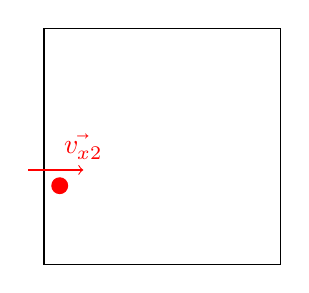
\begin{tikzpicture}
				\draw[black] (0,0) rectangle (3,3);
				\draw[red,fill] (0.2,1) circle (0.1);
				\draw[red,->] (-0.2,1.2) -- (0.5,1.2) node[above]{$\vec{v_{x2}}$};
			\end{tikzpicture}
		\end{multicols}

		На частицу действует сила $F$ со стороны резервуара в течение некоторого времени $\Delta t$, тогда

		\begin{equation*}
			F = \frac{\Delta p}{\Delta t} = \frac{p_1 - p_0}{\Delta t} = \frac{-m_0 v_x - m_0 v_x}{\Delta t} = -\frac{2 m_0 v_x}{\Delta t}.
		\end{equation*}

		В течение времени $\Delta t$ на грань куба площадью $S = a^2$ оказывается давление со стороны частицы

		\begin{equation*}
			P_1 = \frac{\abs{F}}{a^2} = \frac{2 m_0 v_x}{a^2 \Delta t}.
		\end{equation*}

		Так как для каждой отдельной частицы между ее ударами о конкретную стенку проходит время $\Delta t = \frac{2a}{v_x}$, на эту стенку частицей оказывается среднее давление

		\begin{equation*}
			P_0 = P_1 \cdot \frac{\Delta t}{t} = \frac{2 m_0 v_x \cdot v_x \Delta t}{a^2 \d t \cdot 2a} = \frac{m_0 v_x^2}{V}.
		\end{equation*}

		Естественно, такая формула работает и для частиц, двужущихся не только по горизонтали, поскольку движение по трем кооридантным осям в кубе независимо.

		Если просуммировать давление, которое на данную стенку оказывают все частицы, получаем

		\begin{equation*}
			P_x = NP_0 = \frac{N m_0 \langle v_x^2 \rangle}{V} = n m_0 \langle v_x^2 \rangle.
		\end{equation*}

		Здесь $\langle\cdot\rangle$ обозначает среднее по ансамблю. Стоит прокомментировать, почему принцип суперпозиции вообще работает. Мы считаем, что частицы друг с другом взаимодействуют только упруго. Но это означает, что при столкновении двух частиц по каждой из трех осей они либо обе сохраняют свои скорости (что позволяет использовать суперпозицию), либо обмениваются ими, что, с одной стороны, можно интерпретировать как изменение параметров двух частиц, но с другой -- как если бы частицы свободно прошли друг через друга, но при этом поменялись местами. Таким образом, конкретный модуль скорости $\abs{v_x}$ может в разные моменты времени принадлежать разным частицам, но набор всех модулей по всем частицам будет постоянен, поэтому постоянно будет и среднее по ансамблю.

		Это выражение рассматривает давление, приходящееся только на одну из стенок, скажем, левую. По симметрии оно же равно давлению, оказываемому на правую стенку. Аналогично для других направлений. В итоге имеем:

		\begin{align*}
			P_x &= n m_0 \langle v_y^2 \rangle; \\
			P_y &= n m_0 \langle v_y^2 \rangle; \\
			P_z &= n m_0 \langle v_z^2 \rangle.
		\end{align*}

		Поскольку нас интересует давление на все стенки куба, общее давление по определению равно:

		\begin{equation*}
			P = \frac{F}{6S} = \frac{P_x S + P_x S + P_y S + P_y S + P_z S}{6S} = \frac{P_x + P_y + P_z}{3}.
		\end{equation*}

		По теореме Пифагора:

		\begin{equation*}
			\langle v^2 \rangle = \langle v_x^2 + v_y^2 + v_z^2 \rangle,
		\end{equation*}

		что после подстановки в формулу для давления дает

		\namedequation{Основное уравнение МКТ}{P = \frac{1}{3} n m_0 \langle v^2 \rangle}

		Заметим, что для идеальных одноатомных газов (позже мы обсудим, почему это не работает для более сложных газов) кинетическая энергия частиц $E_{k0} = \dfrac{m_0 v^2}{2}$ и потому $P = \dfrac{2}{3} n E_{k0}$.

		Основное уравнение МКТ подтверждается следующим эмперически выведенным законом:

		\namedlaw{Закон Бойля-Мариотта}{При проведении любого процесса над газом при константной температуре, например, сжатии, выполняется: $P_1 V_1 = P_2 V_2$.}
	\end{section}


	\begin{section}{Термодинамическая температура}
		Постараемся осознать, что такое термодинамическая температура. Для этого хочется понять, что такое температура вообще.

		Человек понимает, что есть "горячо" и "холодно". Горячие предметы делают больно. Некоторые предметы более горячие, чем другие: если одну руку положить на горячий предмет, а другую -- на очень горячий, то второй руке станет невыносимо больно раньше. С холодом ситуация аналогичная. Таким образом, можно сделать двустороннюю шкалу холодно-горячо, посередине которой находится человеческое тело. Такая шкала качественная, а не количественная, потому что она не позволяет ответить на вопрос о том, насколько один предмет горячее другого.

		Если горячее тело привести в контакт с холодным, то более горячее тело остынет, а более холодное -- нагреется. Если же в контакт привести одинаково теплые тела, то ни то, не другое не изменит своей ощутимой теплоты. Это упрощает введение температурной шкалы. Достаточно каким-то образом ввести понятие температуры для одного объекта, скажем, дистиллированной воды, а потом отождествить температуру других веществ с такой температурой воды, при которой она с этим веществом входит в тепловое равновесие.

		Как проградуировать температуру для воды? Из опыта мы знаем, что если воду нагревать на горелке, она плавно перейдет из состояния "холодно" (начало опыта) в состояние "горячо" (конец опыта). Состояниям "холодно" и "горячо" придется приписать более или менее условные значения температуры, а значения посередине можно интерполировать линейно: температура в середине опыта (середина -- по времени) будет равна среднему арифметическому начальной и конечных температур и т.д. Для воды разумными реперными точками будет вода сразу после таянья льда -- $0 ^\circ C$ и прямо перед кипением -- $100 ^\circ C$.

		Из опыта мы знаем, что если по железке постучать кувалдой, железка сильно нагреется. Это значит, что работа, совершенная кувалдой, переводится в тепло, то есть теплота -- одна из форм энергии.

		Поскольку горелка постоянно выделяет одно и то же количество теплоты, то есть мощность ее постоянна, то нагрев на единицу температуры требует подведения определенной фиксированной энергии. На что идет эта работа? Зная МКТ, мы понимаем, что единственный возможный вариант -- увеличение кинетической энергии частиц. Таким образом, температура -- мера внутренней энергии частиц вещества.

		Но также из опыта мы знаем, что если нагревать одинаковое время на одной горелке разные вещества, то они нагреются до разных температур. Следовательно, для нагрева вещества на единицу температуры требуется подводить разную энергию, очевидно, пропорциональную массе вещества, но зависящую также и от его вида.

		Однако сама температура по Цельсию не несет физического смысла. Две реперные точки этой шкалы мы выбрали, по сути, случайно. Физический смысл имеет только разность температур, ведь именно она отражает изменение внутренней энергии. Тело при $0 ^\circ C$ не будет иметь нулевую внутреннюю энергию, например, потому что из опыта мы знаем, что лед, то есть воду после кристаллизации, можно охлаждать и дальше.

		Если сместить шкалу Цельсия так, чтобы ноль температуры все же совпадал с нулем внутренней энергии, такая температура будет называться \textbf{термодинамической} и будет пропорциональна внутренней энергии.

		Можно сказать и точнее: термодинамическая температура отражает кинетическую поступательную энергию частиц вещества. Это разумно: за теплопередачу отвечает столкновение частиц, которое приводит к изменению их скоростей, которые, в свою очередь, зависят от кинетических поступательных энергий. Другие же виды энергии, такие как вращательная или колебательная, не вносят вклад в импульс частиц, давление, которое оказывает газ и т.д.

		Из основного уравнения МКТ вытекает, что:

		\begin{equation*}
			\frac{3}{2} \frac{PV}{N} = \frac{m_0 \langle v^2 \rangle}{2},
		\end{equation*}

		причем правая часть этого равенства равна поступательной кинетической энергии частиц, которая, как мы помним, пропорциональна температуре. Следовательно, величина $\frac{PV}{NT}$ -- постоянная для данного вещества.

		Это подтверждается двумя экспериментально открытыми законами:

		\namedlaw{Закон Шарля}{При проведении любого процесса над газом при константном объеме, например, нагреве, выполняется: $\dfrac{P_1}{T_1} = \dfrac{P_2}{T_2}$.}

		\namedlaw{Закон Гей-Люссака}{При проведении любого процесса над газом при константном давлении, например, нагреве, выполняется: $\dfrac{V_1}{T_1} = \dfrac{V_2}{T_2}$.}

		И их обобщением:

		\namedequation{Объединенный газовый закон}{\frac{PV}{T} = \const}

		В нем, естественно, константа пропорциональности зависит не только от рассматриваемого газа, но и от его количества.

		Если провести экспериментальную проверку, например, закона Гей-Люссака, и отметить на графике объем-температура опытные точки, график будет линейным и пересечет ось температур в точке $-273.15 ^\circ C$, являющейся, таким образом, нулем термодинамической шкалы. Для удобства такая смещенная температура выражается не в градусах Цельсия, а в Кельвинах:

		\begin{align*}
			0 K &= -273.15 ^\circ C \\
			1 K &= -272.15 ^\circ C \\
			\dots \\
			273.15 K &= 0 ^\circ C \\
			\dots
		\end{align*}

		Окончательно:

		\definition{Термодинамическая температура $T$ [К]}{мера внутренней энергии частиц вещества; будучи выражена в Кельвинах, смещена от градусов Цельсия на $273.15 ^\circ C$ в положительную сторону}
	\end{section}


	\begin{section}{Уравнение Менделеева-Клапейрона}
		От чего зависит константа пропорциональности $\frac{PV}{NT}$? Понятно, что для одного газа она будет постоянна, но как она различается у разных газов?

		Представим себе камеру в форме прямоугольного параллелепипеда, разделенную поршнем, перпендикулярным горизонтальной оси. Пусть по одну сторону от поршня находится один газ, по другую -- другой, поршень неподвижен (то есть давления уравновешены) и газы находятся в термодинамическом равновесии (то есть имеют одинаковую температуру).

		\tikzsetnextfilename{kmt-temperature1}
		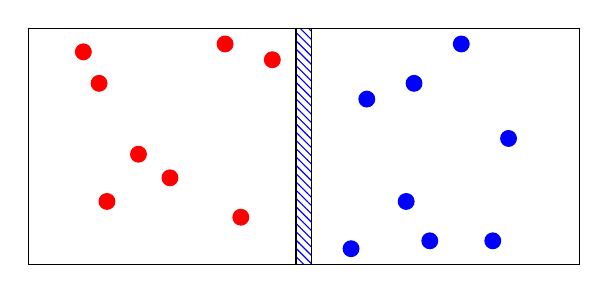
\begin{tikzpicture}
			\draw[black] (0,0) rectangle (7,3);
			\draw[pattern=north west lines, pattern color=blue] (3.4,0) rectangle (3.6,3);

			\draw[red,fill] (1,0.8) circle(0.1);
			\draw[red,fill] (2.7,0.6) circle(0.1);
			\draw[red,fill] (0.9,2.3) circle(0.1);
			\draw[red,fill] (1.4,1.4) circle(0.1);
			\draw[red,fill] (3.1,2.6) circle(0.1);
			\draw[red,fill] (2.5,2.8) circle(0.1);
			\draw[red,fill] (0.7,2.7) circle(0.1);
			\draw[red,fill] (1.8,1.1) circle(0.1);

			\draw[blue,fill] (4.8,0.8) circle(0.1);
			\draw[blue,fill] (5.5,2.8) circle(0.1);
			\draw[blue,fill] (6.1,1.6) circle(0.1);
			\draw[blue,fill] (5.1,0.3) circle(0.1);
			\draw[blue,fill] (4.3,2.1) circle(0.1);
			\draw[blue,fill] (4.9,2.3) circle(0.1);
			\draw[blue,fill] (5.9,0.3) circle(0.1);
			\draw[blue,fill] (4.1,0.2) circle(0.1);

			% \draw[red,fill] (0.2,1) circle (0.1);
			% \draw[red,->] (0.5,1.2) node[above]{$\vec{v_{x1}}$} -- (-0.2,1.2);
		\end{tikzpicture}

		Так как газы имеют одинаковую температуру, они должны иметь постоянную и равную кинетическую поступательную энергию частиц. Иначе говоря, среднее изменение энергии по времени для каждого из газов должно быть равно нулю.

		Рассмотрим упругое столкновение одной из частиц газа массы $m$ с поршнем. Пусть в данный момент поршень массы $M$ движется направо с небольшой скоростью $u$ (да, в среднем поршень неподвижен, но некоторые колебания он претерпевает), а частица имеет скорость $v_x$. Тогда

		\begin{align*}
			mv_x + Mu &= mv_x' + Mu', \\
			\frac{mv_x^2}{2} + \frac{Mu^2}{2} &= \frac{mv_x'^2}{2} + \frac{Mu'^2}{2},
		\end{align*}

		следовательно,

		\begin{align*}
			m(v_x'-v_x) + M(u'-u) &= 0, \\
			m(v_x'^2-v_x^2) + M(u'^2-u^2) &= 0,
		\end{align*}

		откуда путем тривиальных математических преобразований получается

		\begin{equation*}
			u' = \frac{(M - m) u + 2mv_x}{M + m},
		\end{equation*}

		что приводит к изменению кинетической энергии поршня на

		\begin{equation*}
			\Delta E = \frac{Mu'^2 - Mu^2}{2} = \frac{2mM}{(M + m)^2} \left( -M u^2 + m v_x^2 + (M - m) u v_x \right).
		\end{equation*}

		Под термодинамическим равновесием мы понимаем постоянность внутренней энергии в среднем; в моменте, конечно, она может колебаться. Поэтому рассмотрим среднее изменение энергии по времени и приравняем его нулю:

		\begin{equation*}
			\langle \Delta E \rangle = \frac{2mM}{(M + m)^2} \left( -M \langle u^2 \rangle + m \langle v_x^2 \rangle + (M - m) \langle u \rangle \langle v_x \rangle \right) = 0.
		\end{equation*}

		Последний переход от $\langle uv_x \rangle$ к $\langle u \rangle \langle v_x \rangle$ основывается на том, что скорость поршня и скорость частицы можно считать независимыми величинами. Под $\langle v_x^2 \rangle$ понимается не среднее по времени для отдельной частицы, а среднее и по времени, и по ансамблю.

		Поскольку давления газов равны, поршень в среднем неподвижен, и $\langle u \rangle = 0$, что позволяет упростить уравнение до

		\begin{equation*}
			M \langle u^2 \rangle = m \langle v_x^2 \rangle,
		\end{equation*}

		то есть до равенства кинетических энергий поршня и частиц газа по горизонтальной оси.

		Если теперь вспомнить, что по другую сторону поршня находится другой газ, то можно записать аналогичное равенство и по транзитивности получить, что кинетические энергии частиц двух газов по осям X совпадают:

		\begin{equation*}
			\frac{m_1 \langle v_{1x}^2 \rangle}{2} = \frac{m_2 \langle v_{2x}^2 \rangle}{2},
		\end{equation*}

		откуда получается и:

		\begin{equation*}
			\frac{m_1 \langle v_1^2 \rangle}{2} = \frac{m_2 \langle v_2^2 \rangle}{2}.
		\end{equation*}

		Это значит, что термодинамическая температура -- не просто мера внутренней кинетической энергии газа, но и что она прямо пропорциональна кинетической поступательной энергии частиц, и коэффициент пропорциональности -- универсальная константа:

		\begin{equation*}
			\frac{m_0 \langle v^2 \rangle}{2} = \frac{3}{2} kT.
		\end{equation*}

		Коэффициент $k$ называется постоянной Больцмана. Его равенство отношению двух третьих кинетической поступательной энергии к температуре, а не кинетической поступательной энергии к температуре, связано с контекстом, в котором эта константа изначально была определена. Как мы писали ранее, из основного уравнения МКТ вытекает, что:

		\begin{equation*}
			\frac{3}{2} \frac{PV}{N} = \frac{m_0 \langle v^2 \rangle}{2},
		\end{equation*}

		а подставляя сюда формулу для внутренней энергии через температуру, мы получаем:

		\namedlaw{Уравнение Менделеева-Клапейрона}{$PV = NkT$, где $k = \dfrac{R}{N_A} = 1.3806 \cdot 10^{-23} \dfrac{\text{Дж}}{\text{К}}$ -- постоянная Больцмана.}

		Это уравнение является переформулировкой закона, открытого ранее экспериментально:

		\namedlaw{Уравнение состояния идеального газа}{$PV = \nu RT$, где $R = 8.3145 \dfrac{\text{Дж}}{\text{моль}\cdot\text{К}}$ -- универсальная газовая постоянная.}
	\end{section}


	\begin{section}{Степени свободы}
		Как мы уже неоднократно говорили ранее, температура является показателем внутренней кинетической поступательной энергии частиц газа. Что под этим имеется в виду?

		Помимо внутренней кинетической поступательной энергии, отвечающей за скорости частиц, частицы газа обладают другими видами энергии:

		\begin{itemize}
			\item потенциальной энергией частиц, которую мы обсуждали в разделе про агрегатные состояния. Эта энергия высвобождается, когда вещества переходят в более твердые агрегатные вещества;
			\item потенциальной энергией связи, отвечающей за межатомное взаимодействие в молекулах и имеющей в основном электростатическую природу;
			\item кинетической энергией атомов, которая выражаеся в том, что в некоторых случаях атомы могут находится в движении относительно молекул, в которых они находятся;
			\item кинетической вращательной энергией, отвечающей за вращение атомов относительно осей вращения внутри молекул.
		\end{itemize}

		Если бы работа, которую мы подводим к газу, шла на увеличение только кинетической поступательной энергии, то для нагрева одного моля любого вещества на один градус требовалось бы одинаковая работа, но в реальности она тратится также на увеличение других составляющих внутренней энергии газа.

		Оценим вклад отдельных составляющих энергий. Связь между разными видами энергии вычисляется, однако строгий вывод требует подсчета распределений. Мы постараемся привести более или менее интуитивный аргумент, корректный для достаточного количества случаев, подобный тому, который вывел Больцман, не прибегая к подсчету статистики.

		Будем рассматривать столкновение двух частиц массами $m_1, m_2$, движущиеся поступательно со скоростями $\vec{v_1}, \vec{v_2}$ и вращающиеся с угловыми скоростями $\vec{\omega_1}, \vec{\omega_2}$, где направление вектора $\vec{\omega}$ определяется правилом правой руки.

		Должен выполняться закон сохранения энергии:

		\begin{equation*}
			\frac{p_1^2}{2m_1} + \frac{L_1^2}{2I_1} + \frac{p_2^2}{2m_2} + \frac{L_2^2}{2I_2} = \frac{p_1'^2}{2m_1} + \frac{L_1'^2}{2I_1} + \frac{p_2'^2}{2m_2} + \frac{L_2'^2}{2I_2}.
		\end{equation*}

		Путем тривиальных алгебраических преобразования закон сохранения энергии преобразуется к виду

		\begin{multline*}
			\frac{\left( \vec{p_1'} - \vec{p_1} \right) \cdot \left( \vec{p_1'} + \vec{p_1} \right)}{2m_1} + \frac{\left( \vec{L_1'} - \vec{L_1} \right) \cdot \left( \vec{L_1'} + \vec{L_1} \right)}{2I_1} + \\
			+ \frac{\left( \vec{p_2'} - \vec{p_2} \right) \cdot \left( \vec{p_2'} + \vec{p_2} \right)}{2m_2} + \frac{\left( \vec{L_2'} - \vec{L_2} \right) \cdot \left( \vec{L_2'} + \vec{L_2} \right)}{2I_2} = 0.
		\end{multline*}

		Для удобства вычислений (это не обязательное условие) будем считать, что столкновение занимало малое время $\Delta t$, во время которого на первую частицу действовала постоянная сила $\vec{F}$, а на вторую $-\vec{F}$. Тогда можно рассчитать:

		\begin{itemize}
			\item изменение импульсов частиц:
			\begin{align*}
				\vec{p_1'} - \vec{p_1} &= \vec{F} \cdot \Delta t, \\
				\vec{p_2'} - \vec{p_2} &= -\vec{F} \cdot \Delta t,
			\end{align*}

			\item изменение моментов импульсов частиц:
			\begin{align*}
				\vec{L_1'} - \vec{L_1} &= \vec{r} \times \vec{F} \cdot \Delta t, \\
				\vec{L_2'} - \vec{L_2} &= -\vec{r} \times \vec{F} \cdot \Delta t.
			\end{align*}
		\end{itemize}

		Подставляя изменения импульсов и моментов импульсов и деля на $\Delta t$, получаем:

		\begin{equation*}
			\frac{\vec{F}}{m_1} \cdot \left( \vec{p_1'} + \vec{p_1} \right) + \frac{\vec{r} \times \vec{F}}{I_1} \cdot \left( \vec{L_1'} + \vec{L_1} \right) = \frac{\vec{F}}{m_2} \cdot \left( \vec{p_2'} + \vec{p_2} \right) + \frac{\vec{r} \times \vec{F}}{I_2} \cdot \left( \vec{L_2'} + \vec{L_2} \right).
		\end{equation*}

		Для удобства заменим вектор $\vec{F}$ на сонаправленный ему единичный вектор $\vec{f}$, тогда

		\begin{equation*}
			\frac{\vec{f}}{m_1} \cdot \left( \vec{p_1'} + \vec{p_1} \right) + \frac{\vec{r} \times \vec{f}}{I_1} \cdot \left( \vec{L_1'} + \vec{L_1} \right) = \frac{\vec{f}}{m_2} \cdot \left( \vec{p_2'} + \vec{p_2} \right) + \frac{\vec{r} \times \vec{f}}{I_2} \cdot \left( \vec{L_2'} + \vec{L_2} \right),
		\end{equation*}

		причем поскольку частицы могут сталкиваться "боком", возможны практически любые значения $\vec{f}$.

		Пусть $\vec{F} \cdot \Delta t = R \vec{f}$, тогда

		\begin{multline*}
			\frac{\vec{f}}{m_1} \cdot \left( 2 \vec{p_1} + R \vec{f} \right) + \frac{\vec{r} \times \vec{f}}{I_1} \cdot \left( 2 \vec{L_1} + \vec{r} \times R\vec{f} \right) = \\
			= \frac{\vec{f}}{m_2} \cdot \left( 2 \vec{p_2} + R \vec{f} \right) + \frac{\vec{r} \times \vec{f}}{I_2} \cdot \left( 2 \vec{L_2} + \vec{r} \times R\vec{f} \right),
		\end{multline*}

		откуда

		\begin{multline*}
			\frac{R}{m_1} + \frac{R}{I_1} \cdot \left( \vec{r} \times \vec{f} \right)^2 + \frac{2 \vec{f} \cdot \vec{p_1}}{m_1} + \frac{2 \left( \vec{r} \times \vec{f} \right) \cdot \vec{L_1}}{I_1} = \\
			= \frac{-R}{m_2} + \frac{-R}{I_2} \cdot \left( \vec{r} \times \vec{f} \right)^2 + \frac{2 \vec{f} \cdot \vec{p_2}}{m_2} + \frac{2 \left( \vec{r} \times \vec{f} \right) \cdot \vec{L_2}}{I_2}
		\end{multline*}

		и далее

		\begin{equation*}
			R = \frac{2 \vec{f} \cdot \left( \frac{\vec{p_2}}{m_2} - \frac{\vec{p_1}}{m_1} \right) + 2 \left( \vec{r} \times \vec{f} \right) \cdot \left( \frac{\vec{L_2}}{I_2} - \frac{\vec{L_1}}{I_1} \right)}{\frac{1}{m_1} + \frac{1}{m_2} + \left( \frac{1}{I_1} + \frac{1}{I_2} \right) \cdot \left( \vec{r} \times \vec{f} \right)^2}.
		\end{equation*}

		Обозначим числитель этого выражения за $P$, знаменатель -- за $Q$.

		Зная формулу изменения импульса $\vec{p_1'} - \vec{p_1} = R \vec{f}$, можно вычислить новый импульс первой частицы, и похожим образом все другие параметры:

		\begin{equation*}
			\vec{p_1'} = \vec{p_1} + R \vec{f} = \frac{Q \vec{p_1} + P \vec{f}}{Q} = \frac{\left( P + 2 \vec{f} \cdot \frac{\vec{p_1}}{m_1} \right) \cdot \vec{f} + \left( Q \vec{p_1} - \left( 2 \vec{f} \cdot \frac{\vec{p_1}}{m_1} \right) \cdot \vec{f} \right)}{Q}.
		\end{equation*}

		По каждой из осей:

		\begin{equation*}
			p_{1x}' = \frac{\left( P + 2 \vec{f} \cdot \frac{\vec{p_1}}{m_1} \right) \cdot f_x + \left( Q p_{1x} - \left( 2 \vec{f} \cdot \frac{\vec{p_1}}{m_1} \right) \cdot f_x \right)}{Q}.
		\end{equation*}

		В выражении $P + 2 \vec{f} \cdot \frac{\vec{p_1}}{m_1}$ часть, зависящая от $\vec{p_1}$, сокращается. Для независимых величин со средним значением $0$ выполняется:

		\begin{equation*}
			x = \sum_{i=1}^n x_i \implies \langle x^2 \rangle = \sum_{i=1}^n \langle x_i^2 \rangle.
		\end{equation*}

		Это равенство легко проверить, воспользовавшись линейностью математического ожидания и формулой для произведения математических ожиданий независимых величин.

		В нашем случае по каждой из координат:

		\begin{equation*}
			\langle p_{1x}'^2 \rangle = \frac{\left\langle \left( P + 2 \vec{f} \cdot \frac{\vec{p_1}}{m_1} \right)^2 \right\rangle \cdot f_x^2 + \left\langle \left( Q p_{1x} - \left( 2 \vec{f} \cdot \frac{\vec{p_1}}{m_1} \right) \cdot f_x \right)^2 \right\rangle}{Q^2}.
		\end{equation*}

		В частности, по оси, направленной по вектору $\vec{f}$:

		\begin{equation*}
			\langle p_{1f}'^2 \rangle = \frac{\left\langle \left( P + 2 \frac{p_{1f}}{m_1} \right)^2 \right\rangle + \left( Q - \frac{2}{m_1} \right)^2 \cdot \langle p_{1f}^2 \rangle}{Q^2}.
		\end{equation*}

		Так как газ находится в равновесии, $\langle p_{1f}'^2 \rangle = \langle p_{1f}^2 \rangle$, тогда:

		\begin{equation*}
			4 \left( Q - \frac{1}{m_1} \right) \cdot \frac{1}{m_1} \cdot \langle p_{1f}^2 \rangle = \left\langle \left( P + 2 \frac{p_{1f}}{m_1} \right)^2 \right\rangle.
		\end{equation*}

		Раскрывая $P$ и $Q$:

		\begin{multline*}
			\left( \frac{1}{m_2} + \left( \frac{1}{I_1} + \frac{1}{I_2} \right) \cdot \left( \vec{r} \times \vec{f} \right)^2 \right) \cdot \frac{1}{m_1} \cdot \langle p_{1f}^2 \rangle = \\
			= \left\langle \left( \vec{f} \cdot \frac{\vec{p_2}}{m_2} + \left( \vec{r} \times \vec{f} \right) \cdot \left( \frac{\vec{L_2}}{I_2} - \frac{\vec{L_1}}{I_1} \right) \right)^2 \right\rangle = \\
			= \left\langle \left( \vec{f} \cdot \frac{\vec{p_2}}{m_2} \right)^2 \right\rangle + \left\langle \left( \left( \vec{r} \times \vec{f} \right) \cdot \frac{\vec{L_1}}{I_1} \right)^2 \right\rangle + \left\langle \left( \left( \vec{r} \times \vec{f} \right) \cdot \frac{\vec{L_2}}{I_2} \right)^2 \right\rangle.
		\end{multline*}

		Путем алгебраических преобразований получаем:

		\begin{multline*}
			\frac{1}{m_2} \cdot \left( \frac{\langle p_{1f}^2 \rangle}{m_1} - \frac{\langle p_{2f}^2 \rangle}{m_2} \right) \\
			+ \frac{\left( \vec{r} \times \vec{f} \right)^2}{I_1} \cdot \left( \frac{\langle p_{1f}^2 \rangle}{m_1} - \frac{\langle L_{1rf}^2 \rangle}{I_1} \right) \\
			+ \frac{\left( \vec{r} \times \vec{f} \right)^2}{I_2} \cdot \left( \frac{\langle p_{1f}^2 \rangle}{m_1} - \frac{\langle L_{1rf}^2 \rangle}{I_2} \right) = 0,
		\end{multline*}

		где за $v_{rf}$ обозначается проекция вектора $\vec{v}$ на ось $\vec{r} \times \vec{f}$.

		Поскольку величины $p_f$, $L_{rf}$, $\vec{r}$ и $\vec{f}$ могут принимать самые различные значения, а равенство должно выполняться всегда, то должно быть равно нулю каждое из слагаемых, то есть:

		\begin{align*}
			\frac{\langle p_{1f}^2 \rangle}{m_1} &= \frac{\langle p_{2f}^2 \rangle}{m_2}, \\
			\frac{\langle p_{1f}^2 \rangle}{m_1} &= \frac{\langle L_{1rf}^2 \rangle}{I_1}, \\
			\frac{\langle p_{1f}^2 \rangle}{m_1} &= \frac{\langle L_{1rf}^2 \rangle}{I_2},
		\end{align*}

		а это есть ничто иное, как равенство энергий различных форм, за исключением того, что рассматриваются проекции векторов на некоторые оси.

		Постараемся осознать полученный нами результат.

		Ранее мы показали, что

		\begin{equation*}
			\frac{m_0 \langle v^2 \rangle}{2} = \frac{3}{2} kT.
		\end{equation*}

		Поскольку по теореме Пифагора $v^2 = v_x^2 + v_y^2 + v_z^2$, это можно переписать как

		\begin{equation*}
			\frac{m_0 \langle v_x^2 \rangle}{2} = \frac{kT}{2},
		\end{equation*}

		что можно интерпретировать как тот факт, что каждая из переменных $v_x, v_y, v_z$ запасает по $\frac{kT}{2}$ энергии. Из выведенной системы мы понимаем, что и

		\begin{equation*}
			\frac{I_0 \langle \omega_x^2 \rangle}{2} = \frac{kT}{2},
		\end{equation*}

		то есть каждая из переменных $\omega_x, \omega_y, \omega_z$ запасает по $\frac{kT}{2}$ энергии.

		Кроме того, наше доказательство было удивительно алгебраичным. Физическая информация закодирована только в том, что формула для энергии по каждой из переменных имеет вид $\lambda x^2$. Вообще говоря, мы не опирались даже на второй закон Ньютона или формулу изменения моментов импульсов: выражение $\vec{r} \times \vec{F} \cdot \Delta t$ как было введено вначале, так и осталось до конца как $\vec{r} \times \vec{f}$. Это значит, что выведенный закон гораздо более универсален: он связывает не просто кинетические поступательную и вращательную энергию, а вообще все виды энергии, зависящие от переменной квадратично.

		Таким образом, каждый из параметров, описывающих частицу, вносит вклад в ее энергию, равный $\frac{kT}{2}$. Это включает как уже знакомые нам три координаты поступательной и вращательной скорости, так и более сложные величины. Количество таких чисел называется числом \textbf{степеней свободы} и обозначается $i$.

		\namedlaw{Теорема о равнораспределении}{На каждую степень свободы приходится энергия $\frac{kT}{2}$.}

		Таким образом, общая энергия газа равна

		\begin{equation*}
			E = \frac{ikT}{2}.
		\end{equation*}

		Здесь стоит сделать важный комментарий. Необходимым условием для работы теоремы о равнораспределении является то, что разные виды энергии могут переходить друг в друга. Мы неявно пользовались этим при ее выводе, когда предполагали, что столкновения частиц бывают нецентральными, и частицы при этом будут закручиваться.

		В реальности в этом месте возникает проблема. Экспериментальное число степеней свободы для одноатомных газов -- три, что соответствует поступательному движению по трем осям. Отсюда мы делаем вывод о том, что атомы не могут вращаются. Это достаточно разумно: если представлять себе атомы как материальные точки, то они обязаны иметь нулевой момент инерции относительно собственной оси, а если как шары микроскопического размера, то для придания им вращательной энергии $\frac{kT}{2}$ пришлось бы разогнать их до огромных скоростей, при которых начались бы веселые явления вроде излучения.

		Для двухатомных газов можно применить ту же логику. Каждая частицы двухатомного газа содержит по два атома со связью между ними. Это значит, что каждый атом вносит по три поступательные степени свободы, плюс есть потенциальная энергия связи, итого семь степеней свободы. Энергия вращения не рассматривается отдельно, поскольку она уже учтена в относительном движении атомов.

		Вычисленные нами семь степеней свободы можно проинтерпретировать и чуть иначе: три степени свободы отвечают за поступательное движение центра масс, две -- за вращение вокруг двух осей (вращение вокруг оси связи невозможно подобно тому, как невозможно вращение атома вокруг своей оси), одна -- за движение атомов по оси связи в противоположные стороны, то есть вибрацию, и одна -- за саму связь.  Если связь в двухатомной частице не прочная, а может удлиняться и сжиматься, подобно пружинному маятнику, то действительно необходимо учесть возможность колебаний. Мы учитываем связь в некотором смысле дважды, как вибрационное движение атомов и как потенциальную энергию, поскольку маятник обладает и кинетической энергией, соответствующей мгновенной скорости атомов относительно связи, и потенциальной энергией, заключенной в самой связи, где нулем энергии считается точка равновесия связи.

		Однако экспериментальное значение оказывается равным $i = 5$. Дело в том, что при обычных температурах связь не может изменить свою длину. Это автоматически накладывает ограничение на скорость атомов относительно связи -- ноль, и на энергию связи -- также ноль (относительно точки равновесия). При низких температурах оказывается, что $i = 3$, что соответствует запрету на вращение частицы. Так проявляется \textbf{вымораживание степеней свободы}.

		Причина вымораживания заключается в квантовомеханической природе вещества. Квантовая механика требует квантования момента импульса. Это значит, что энергия вращения не может вноситься в частицы за счет столкновений постепенно в течении долгого времени, а долна изменяться рывками. При низких температурах частицы движутся настолько медленно, что изменение момента импульса, вычисленное классически, много меньше шага квантования, поэтому столкновения не могут создавать вращательное движение.

		Правильнее считать, таким образом, что у частиц всех газов, даже одноатомных, присутствуют все степени свободы: три кинетические поступательные, три кинетические вращательные, и по одной кинетической и потенциальной колебательной на каждую связь.

		В случае одноатомных газов вращательные степени свободы вымораживаются при всех практически реальных температурах. В случае двухатомных газов вымораживается только одна вращательная степень свободы, коллинеарная связи. Выморожены ли две колебательные степени свободы, зависит от температуры; при нормальных условиях в большинстве двухатомных газов они не активированы, потому обычно считается, что двухатомные газы имеют пять степеней свободы. Частицы многоатомного ($\ge 3$) газа при обычных температурах имеют шесть степеней свободы: три кинетических поступательных и три вращательных, а все вибрационные степени свободы выморожены.

		\def\arraystretch{2.5}
		\begin{tabular}{c|c|c}
			& Количество степеней свободы & Полная внутренняя энергия \\ \hline
			Одноатомный газ & $i = 3$ & $E = \dfrac{3kT}{2}$ \\
			Двухатомный газ & $i = 5$ & $E = \dfrac{5kT}{2}$ \\
			Многоатомный газ & $i = 6$ & $E = \dfrac{6kT}{2}$
		\end{tabular}
	\end{section}


	\begin{section}{Теплоемкость}
		Мы уже говорили о том, что температура является мерой кинетической поступательной энергии частиц тела, но при этом энергия, которая идет на нагрев тела, распределяется по всем видам энергий. Таким образом, на нагрев тела на температуру $\Delta T$ требуется $\frac{i}{2} k \Delta T = \frac{i}{2} \nu R \Delta T$ энергии. Эта формула выполняется точно только для идеальных газов, однако основополагающее утверждение о том, что температура прямо пропорциональна кинетической поступательной энергии, которая, в свою очередь, прямо пропорциональна полной внутренней энергии, остается. Это означает, что на нагрев определенного вещества на единицу температуры всегда требуется одно и то же количество энергии.

		\definition{Теплоемкость}{количество теплоты, которое получает тело при нагревании на единицу температуры}

		\namedequation{Теплоемкость $C$ [Дж/К]}{C = \frac{\delta Q}{\delta T}}

		Поскольку теплоемкость, очевидна, прямо пропорциональна количеству частиц тела, выделяют также:

		\namedequation{Удельная теплоемкость $c$ [Дж/кг $\cdot$ К]}{c = \frac{C}{m} = \frac{\delta Q}{m \delta T}}

		\namedequation{Молярная теплоемкость $c$ [Дж/моль $\cdot$ К]}{c = \frac{C}{\nu} = \frac{\delta Q}{\nu \delta T}}

		Частицы твердых тел в первом приближении могут колебаться в трех направлениях, задаваемых кристаллической решеткой, и каждое из этих направлений задает две степени свободы: одна кинетическая и одна потенциальная, -- потому для твердых тел $c_{\text{молярная}} \approx 3R$.

		Понятие теплоемкости, вообще говоря, не учитывает то, каким путем произошел нагрев тела. Выражение $\delta Q$ является функцией процесса и зависит от того, каким путем менялись объем, давление и температура при нагреве. Поэтому для газов выделяют:

		\namedequation{Молярная теплоемкость при постоянном объеме}{c_V = \frac{(i/2) \nu R \d T}{\nu \d T} = \frac{i}{2} R}

		\namedequation{Молярная теплоемкость при постоянном давлении}{c_P = \frac{((i+2)/2) \nu R \d T}{\nu \d T} = \frac{i + 2}{2} R}

		Вывод этих значений будет приведен ниже в разделе о изопроцессах.

		Удельные и молярные теплоемкости -- табличные величины, помогающие решать задачи на теплоту. Так, в замкнутых системах выполняется закон сохранения энергии:

		\begin{equation*}
			\sum_i c_i m_i (T_{i1} - T_{i0}) = 0,
		\end{equation*}

		что позволяет решать простейшие задачи в духе "какова температура двух проконтактировавших тел после достижения термодинамического равновесия".
	\end{section}


	\begin{section}{Агрегатные состояния возвращаются}
		Если твердое тело нагревать до высоких теператур, в какой-то момент оно превратится в жидкость. Если его нагревать дальше, оно превратится в газ. Из опыта мы знаем, что например, вода, образовавшаяся от только что растаявшего льда, имеет ту же температуру, что и лед, из которого она образовалась. Таким образом, подведенная к телу энергия тратится попеременно то на увеличение температуры (то есть кинетической энергии частиц), то на изменение агрегатного состояния (то есть увеличение потенциальной энергии частиц).

		Для переходов между агрегатными состояниями вводятся специальные понятия:

		\def\arraystretch{2.5}
		\begin{tabular}{c|c|c|c}
			& Из твердого тела & Из жидкости & Из газа \\ \hline
			В твердое тело & -- & Кристаллизация & Десублимация \\
			В жидкость & Плавление & -- & Конденсация \\
			В газ & Возгонка/сублимация & Испарение & --
		\end{tabular}

		Естественно, при обычных условиях возможны только переходы между соседними агрегатными состояниями, то есть возгонка и десублимация невозможны. О том, когда это все-таки происходит, поговорим чуть позже.

		\definition{Температура плавления}{граничная температура между твердым телом и жидкостью, то есть та температура, при которой вещество может одновременно существовать в твердой и жидкой форме}

		\definition{Температура парообразования}{граничная температура между жидкостью и газом, то есть та температура, при которой вещество может одновременно существовать в жидкой и газообразной форме}

		То, что эти понятия называются именно так, а не, скажем, температура кристаллизации или конденсации соответственно -- не более, чем историческая особенность. Исключение составляют аморфные вещества, в которых нельзя провести линию между твердой и жидкой формой. В этом случае температурой кристаллизации условно называют температуру, при которой тело практически полностью теряет качества жидкости, а температурой плавления -- температурой, при которой оно теряет качества твердого тела.

		\definition{Удельная теплота плавления $\lambda$ [Дж/кг]}{теплота, необходимая для плавления единицы массы вещества}

		\definition{Удельная теплота парообразования $L$ [Дж/кг]}{теплота, необходимая для испарения единицы массы вещества}

		Это также табличные величины. С названиями ситуация такая же, как и с названиями температур.
	\end{section}


	\begin{section}{Влажность и пар}
		Если в замкнутый резервуар налить воду, она начнет немного испаряться. Это связано с тем, что не все частицы жидкости обладают одной и той же энергией: в нем есть частицы с энергией, как большей средней, так и меньшей. Самые быстрые частицы имеют кинетическую энергию, достаточную для того, чтобы покинуть жидкость. Таким образом, в резервуаре одновременно сосуществуют газ и жидкость, даже если температура меньше температуры плавления. Это явление называется \textbf{испарением}.

		В то же время происходит и обратный процесс: частицы газа могут захватываться жидкостью. В какой-то момент будет достигнуто равновесие, скорость конденсации будет равна скорости испарения. Такое состояние равновесия называется \textbf{насыщенным паром}.

		\definition{Насыщенный пар}{пар, находящийся в динамическом равновесии с жидкостью: в единицу времени испаряется столько же пара, сколько конденсируется}

		Соответственно, состояние между нулевым количеством пара и насыщенным паром называется \textbf{ненасыщенным паром}:

		\definition{Ненасыщенный пар}{пар, количество которого в моменте растет за счет испарения жидкости}

		Пар в незамкнутом сосуде всегда ненасыщен. В замкнутом сосуде жидкость сначала будет испаряться, образуя ненасыщенный пар, а затем, когда пара испарится достаточно много, он станет насыщенным.

		Поскольку удаление из жидкости быстрых молекул способствует уменьшению средней кинетической энергии частиц и, следовательно, температуры, испарение сопровождается понижением температуры жидкости, что, в свою очередь, приводит к замедлению испарения. Кстати отметим, что, поскольку испарение обусловлено высокими скоростями отдельных частиц, оно сильно ускоряется при ветре.

		Анализ системы жидкость-пар даже в равновесии затруднен, поскольку система состоит из двух частей, одна из которых имеет постоянный объем, а другая -- переменный. Тем не менее, некоторые общие результаты получить возможно.

		Рассмотрим резервуар, на дне которого находится жидкость, а остальной объем занимает насыщенный пар. Если объем резервуара увеличивать, сохраняя температуру, газ будет занимать больший объем пространства, и, следовательно, молекулы газа реже будут переходить в жидкость, и равновесие нарушится. Чтобы равновесие сохранилось, частота конденсации должна быть постоянной. Макроскопически это означает, что постоянной должна быть сила давления пара.

		Посмотрим, что случится при изменении геометрии резервуара. Если изменять площадь контакта жидкости и пара, сохраняя при этом объем и температуру, то количество высокоскоростных частиц на контактной поверхности будет изменяться пропорционально, и поэтому пропорционально будет меняться частота конденсации. Для сохранения динамического равновесия пропорционально должна измениться и сила давления пара $F_P = PS$. Следовательно, давление пара должно быть постоянно.

		Пропорциональное изменения количества насыщенного пара и жидкости, естественно, равновесие не нарушит.

		Таким образом, при постоянной температуре независимо от количества вещества, геометрии резервуара и других параметров давление насыщенного газа является постоянной величиной. Зависимость давления насыщенного пара от температуры -- табличная величина.

		Для водяного пара в воздухе вводят отдельные понятия:

		\namedequation{Относительная влажность воздуха $\varphi$ [\%]}{\varphi = \frac{P_{\text{текущего вод. пара}}}{P_{\text{насыщен. вод. пара}}} \cdot 100\%}

		Под давлением насыщенного водяного пара понимается то давление, которым обладал бы насыщенный водяной пар при текущей температуре. Таким образом, нулевая влажность воздуха означает, что водяного пара нет, 100\%-я -- что водяной пар насыщен (а не то, что воздух целиком превратился в воду).

		С ростом температуры давление насыщенного пара повышается. Это обусловлено тем, что при повышении температуры большая доля частиц жидкости получают кинетическую энергию, достаточную для испарения.

		Наоборот, если понижать температуру системы с ненасыщенным паром, то жидкость будет отдавать все меньшую долю частиц на испарение, и будет достигнуто состояние насыщенного пара.

		\definition{Точка росы}{температура, при которой данный водяной пар становится насыщенным ($\varphi = 100\%$) и начинает конденсироваться. Иначе: такая температура, что давление насыщенного пара при этой температуре равно текущему давлению данного пара (при текущей температуре)}

		При исследовании газов под давлениями, близкими к давлениям насыщенного пара данного вещества, нередко нужно учитывать возможную конденсацию при уменьшении температуры или увеличении давления. Например, водяной пар в замкнутом объеме с относительной влажностью $60\%$ при изотермическом уменьшении объема в два раза по закону Бойля-Мариотта $PV = \const$ должен был бы увеличить свое давление в два раза, а значит и увеличить относительную влажность до $120\%$. Однако относительная влажность не может превышать $100\%$, значит часть жидкости сконденсировалась, и в сосуде сосуществуют жидкость и газ под давлением насыщенного пара. Зная давление насыщенного пара, его температуру и предположив, что объем жидкости мал по сравнению с объемом сосуда, можно использовать уравнение состояния идеального газа, чтобы рассчитать количество вещества пара и таким образом вычислить параметры и воды, и пара.

		При анализе систем на практике часто пригождается одно из следствий постулатов МКТ. Поскольку мы считаем, что частицы газа не контактируют друг с другом, то два газа, находящиеся в одной области пространства, оказывают на нее эффект, равный сумме эффектов, оказываемых каждым из газов в отдельности:

		\namedlaw{Закон Дальтона}{Давление нескольких идеальных газов в одном объеме равно сумме давлений, оказываемых газами по отдельности (\textbf{парциальных давлений})}
	\end{section}


	\begin{section}{Фазовая диаграмма}
		Для того, чтобы проще представлять себе состояния веществ при разных параметрах, используют фазовые диаграммы. Классическая фазовая диаграмма -- график от давления и температуры, в котором для каждой точки указано агрегатное состояние, в котором существует вещество при этих параметрах.

		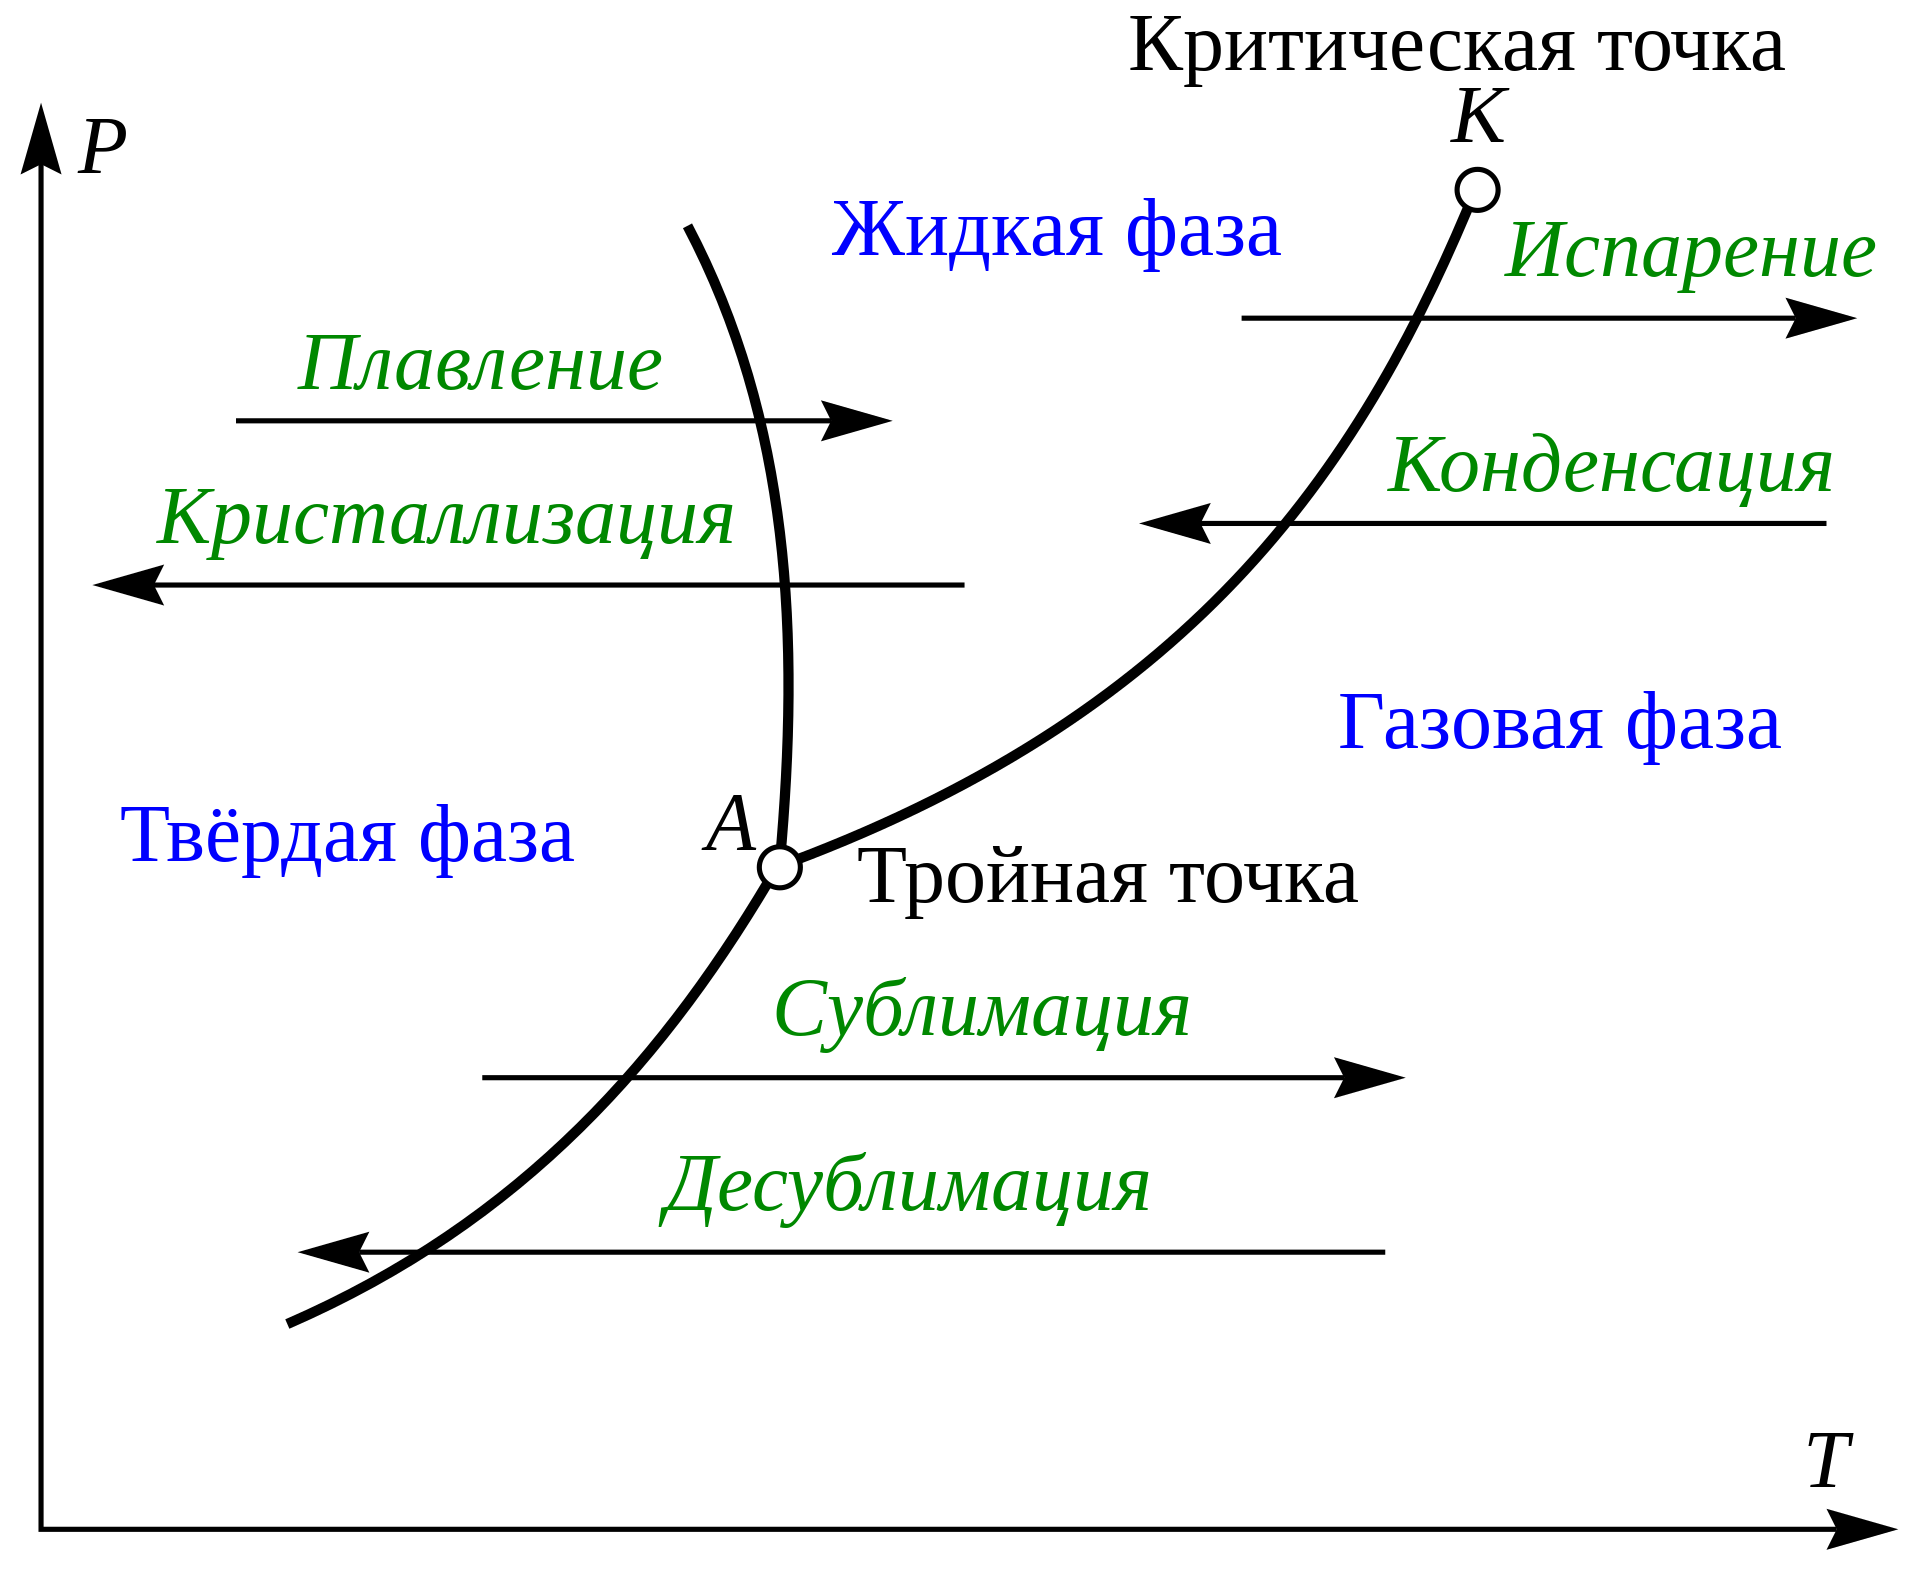
\includegraphics[width=\textwidth]{images/phasediagram1.png}

		Кривые линии обозначают состояния, при которых могут сосуществовать разные агрегатные состояния. Сейчас мы обсудим, откуда появляется фазовая диаграмма и почему она имеет именно такой вид.

		Для начала полезно подумать над тем, как температуры плавления и испарения зависят от давления.

		Увеличение давления приводит к повышению плотности вещества, то есть его частицы приближаются друг к другу. Если вещество находится в твердом агрегатном состоянии, это приводит к увеличению взаимодействия между молекулами, кристаллическая решетка становится более упругой. Соответственно, для перехода между соседними клетками решетки частицам необходима несколько большая кинетическая энергия, то есть температура плавления увеличивается. Аналогичная ситуация происходит и с температурой парообразования.

		Вода и немногие другие вещества -- удивительные исключения из этого закона. Кристаллическая структура льда формируется за счет водородных связей, выстраивающих молекулы воды в решетку. При кристаллизации молекулы воды ориентируются особым образом друг относительно друга, и каждой молекуле энергетически выгоднее оказывается связаться с четырьмя другими молекулами (этот же эффект ответственен за меньшую плотность льда, чем у воды). При увеличении давления молекулы воды сближаются, и эта структура начинает ломаться, предпочитая жидкость твердой фазе. Таким образом, с увеличением давления для плавления требуется все меньшая температура.

		Чтобы проанализировать, что происходит при повышении давления дальше, представим себе жидкость, находящуюся в динамическом равновесии со своим насыщенным паром. При повышении давления и температуры так, чтобы температура была равна температуре плавления при текущем давлении, частицы жидкости будут иметь все большие энергии и следовательно, требовать для сохранения структуры все больше объема, что приведет к понижению плотности жидкости. В то же время все больше частиц будут испаряться, что приведет к повышению плотности газа. В какой-то момент эти плотности сравняются, но это означает, что мы больше не можем говорить о сосуществовании газа и жидкости. Таким образом, начиная с какого-то момента жидкость и газ ставновятся неразличимыми.

		\definition{Критическая точка}{точка фазовой диаграммы на кривой парообразования, в которой газ и жидкость становятся неразличимыми}

		Посмотрим теперь, что происходит при низких давлениях. Мы знаем, что в твердых телах частицы обладают недостаточной кинетической энергией для того, чтобы "перескочить" между клетками кристаллической решетки. Если повысить температуру до того уровня, при котором это возможно, вещество станет жидким. Однако если давление мало настолько, что на поверхностные частицы вещества внешняя сила оказывается меньше, чем сила отталкивания со стороны других частиц вещества, то вещество тут же испарится, "перескакав" через жидкую фазу. Это значит, что при низких давлениях фазовый переход возможен между твердым телом и газом напрямую.

		Если при больших давлениях температура парообразования превышает температуру плавления, а при меньших они совпадают, то на фазовой диаграмме обязана существовать так называемая \textbf{тройная точка}, в которой кривые парообразования и плавления пересекаются. В тройной точке вещество может сосуществовать сразу в трех агрегатных состояниях.

		\definition{Тройная точка}{точка фазовой диаграммы на кривой парообразования, в которой могут сосуществовать твердая, жидкая и газообразная фаза одного вещества}

		Более полная фазовая диаграмма, указывающая на свойства вещества, выглядит следующим образом:

		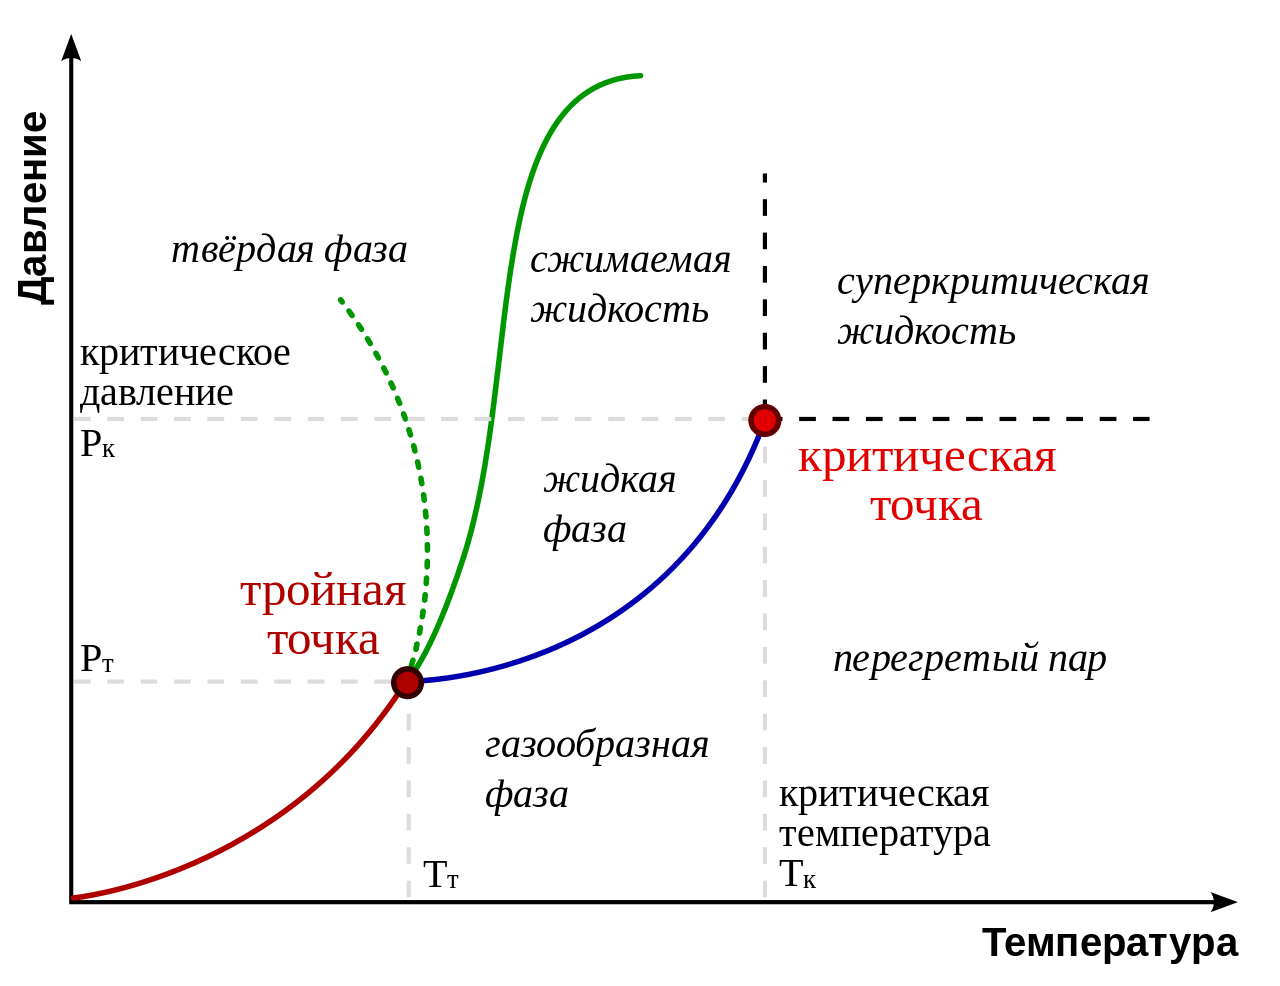
\includegraphics[width=\textwidth]{images/phasediagram2.png}

		Здесь сплошная зеленая линия показывает кривую плавления для большинства веществ, пунктирная зеленая линия -- аномальную кривую плавления воды.
	\end{section}


	\begin{section}{Распределение Максвелла}
		Как нам известно, средняя кинетическая поступательная энергия частиц газа равна $\frac{3}{2} kT$, но пока мы ничего не знаем о том, какая доля частиц имеет какую энергию и скорость.

		Пусть $f(v) \d v$ -- доля частиц, у которых проекция скорости на ось $x$ оежит в диапазоне от $v$ до $v + \d v$. Тогда

		\begin{equation*}
			\int_{-\infty}^{+\infty} f(v) \d v = 1.
		\end{equation*}

		Пусть $g(\vec{v}) \d v_x \d v_y \d v_z$ -- доля частиц, имеющих проекции скоростей на оси $x, y, z$ от $v_x, v_y, v_z$ до $v_x + \d v_x, v_y + \d v_y, v_z + \d v_z$ соответственно.

		Будем считать проекции скоростей на оси $x, y, z$ независимыми величинами, тогда

		\begin{equation*}
			g(\vec{v}) \d v_x \d v_y \d v_z = f(v_x) \d v_x \cdot f(v_y) \d v_y \cdot f(v_z) \d v_z \implies g(\vec{v}) = f(v_x) f(v_y) f(v_z).
		\end{equation*}

		Будем также считать, что скорости распределены по направлениям равномерно, то есть вероятность найти частицу в данном диапазоне модулей скоростей не зависит от того, какой диапазон направлений скоростей мы исследуем. Это означает, что величина $g(\vec{v})$ зависит только от $v$, а не от направления вектора скорости.

		Тогда, в частности,

		\begin{equation*}
			f \left( \sqrt{v_x^2 + v_y^2 + v_z^2} \right) f(0) f(0) = f(v_x) f(v_y) f(v_z).
		\end{equation*}

		С этого момента физика заканчивается и начинается математика.

		Пусть $h(v^2) = \ln \lambda f(v)$, причем $\lambda$ выбрано так, что $h(0) = 0$, тогда уравнение выше можно упростить до

		\begin{equation*}
			h \left(v_x^2 + v_y^2 + v_z^2 \right) = h \left(v_x^2 \right) + h \left(v_y^2 \right) + h \left(v_z^2 \right).
		\end{equation*}

		Общим решением уравнения такого вида является $h(v^2) = \nu v^2$ для некоторого $\nu$, отсюда

		\begin{equation*}
			f(v) = \frac{1}{\lambda} e^{\nu v^2}.
		\end{equation*}

		Доля частиц обязана убывать с возрастанием скорости, поскольку иначе средняя скорость была бы бесконечно, поэтому $\nu < 0$. Сделаем замену $\nu = -\frac{1}{\alpha^2}$, тогда

		\begin{equation*}
			f(v) = \frac{1}{\lambda} e^{-\frac{v^2}{\alpha^2}}.
		\end{equation*}

		Условие на единичность интеграла:

		\begin{equation*}
			1 = \int_{-\infty}^{+\infty} f(v) \d v = \frac{\alpha \sqrt{\pi}}{\lambda},
		\end{equation*}

		откуда $\lambda = \alpha \sqrt{\pi}$ и далее

		\begin{equation*}
			f(v) = \frac{1}{\alpha \sqrt{\pi}} e^{-v^2 / \alpha^2}.
		\end{equation*}

		Это выражение описывает распределение проекций $v_x$. Для вектора скорости имеем

		\begin{equation*}
			g(\vec{v}) = f(v_x) f(v_y) f(v_z) = \frac{1}{\left( \alpha \sqrt{\pi} \right)^3} e^{-(v_x^2 + v_y^2 + v_z^2) / \alpha^2} = \frac{1}{\alpha^3 \pi \sqrt{\pi}} e^{-v^2 / \alpha^2}.
		\end{equation*}

		Введя функцию $g'(v, \theta, \phi)$ для сферических координат аналогично $g$, получаем связь:

		\begin{equation*}
			g'(v, \theta, \phi) \d v \d \theta \d \phi = g(\vec{v}) v^2 \sin \theta \d v \d \theta \d \phi.
		\end{equation*}

		Таким образом, доля $p(v) \d v$ частиц, имеющих модуль скорости от $v$ до $v + \d v$, равна

		\begin{align*}
			p(v) \d v &= \int_0^\pi \left( \int_0^{2\pi} g'(v, \theta, \phi) \d \phi \right) \d \theta \d v \\
			&= \int_0^\pi \left( \int_0^{2\pi} g(\vec{v}) v^2 \sin \theta \d \phi \right) \d \theta \d v \\
			&= \frac{1}{\alpha^3 \pi \sqrt{\pi}} v^2 e^{-v^2/\alpha^2} \int_0^\pi \left( \int_0^{2\pi} \sin \theta \d \phi \right) \d \theta \d v \\
			&= \frac{4}{\alpha^3 \sqrt{\pi}} v^2 e^{-v^2/\alpha^2} \d v.
		\end{align*}

		Самая вероятная скорость достигается при

		\begin{equation*}
			\frac{\d p}{\d v_{max}} = 0 \iff v_{max} = \alpha.
		\end{equation*}

		Средний модуль скорости частиц

		\begin{equation*}
			\langle v \rangle = \int_{0}^{+\infty} v p(v) \d v = \int_0^{+\infty} \frac{4}{\alpha^3 \sqrt{\pi}} v^3 e^{-v^2 / \alpha^2} \d v = \frac{2 \alpha}{\sqrt{\pi}} \int_0^{+\infty} t e^{-t} \d t = \frac{2 \alpha}{\sqrt{\pi}},
		\end{equation*}

		а средний квадрат скорости

		\begin{equation*}
			\langle v^2 \rangle = \int_0^{+\infty} v^2 p(v) \d v = \int_0^{+\infty} \frac{4}{\alpha^3 \sqrt{\pi}} v^4 e^{-v^2 / \alpha^2} \d v = \frac{4 \alpha^2}{\sqrt{\pi}} \int_0^{+\infty} t^4 e^{-t^2} \d t = \frac{3 \alpha^2}{2}.
		\end{equation*}

		Комбинируя это равенство с формулой, связывающей энергию с температурой, получаем

		\begin{equation*}
			\alpha = \sqrt{\frac{2kT}{m_0}}.
		\end{equation*}

		Таким образом:

		\begin{equation*}
			v_{max} = \sqrt{\frac{2kT}{m_0}}, \qquad
			\langle v \rangle = \sqrt{\frac{8kT}{\pi m_0}}, \qquad
			\langle v^2 \rangle = \frac{3kT}{m_0}. \\
		\end{equation*}

		График $p(v)$ имеет вид:

		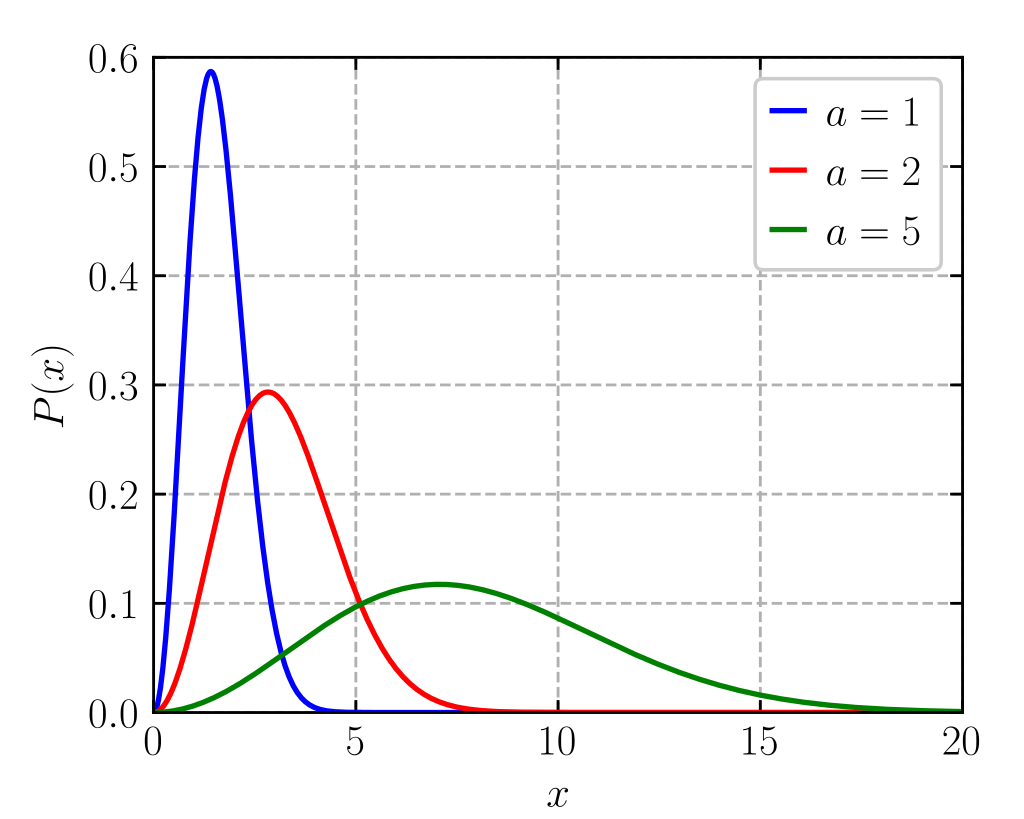
\includegraphics[width=\textwidth]{images/maxwelldistribution.png}

		Здесь единицы условны, большее значение $a$ соответствует большей температуре.
	\end{section}


	\begin{section}{Начала термодинамики}
		После того, как мы провели столько теоретических вычислений и описали столько термодинамических эффектов, можно подвести некоторый промежуточный итог и отметить, какими эмперическими утверждениями мы при этом пользовались.

		Такие утверждения называют \textbf{началами термодинамики}, подобно аксиомам в математике. Эти утверждения универсальны, выполняются для всех тел и не зависят от используемой модели: многие начала были введены, когда еще использовалась теплородная теория.

		Первые два начала утверждают существование термодинамического равновесия и то, что любая система к нему приходит. Ими мы пользовались, например, когда получали распределение Максвелла чисто математически, используя симметрии.

		\namedlaw{Общее (минус первое) начало термодинамики}{Вне зависимости от начального состояния изолированной системы, в конце концов, в ней установится термодинамическое равновесие, и все части системы при достижении этого равновесия будут иметь одинаковую температуру.}

		\namedlaw{Нулевое начало термодинамики}{Существует некоторый макроскопический параметр термодинамических систем, называемый температурой, такой что любые две системы с одинаковой температурой находятся в термодинамическом равновесии и наоборот.}

		Следующее начало указывает на связь температуры и внутренней энергии и на энергетическую природу теплоты.

		\namedlaw{Первое начало термодинамики}{Подведенное к телу количество теплоты идет на увеличение внутренней энергии этого тела и совершение этим телом работы: $Q = \Delta U + A_{\text{газа}}$.}

		Здесь под количеством теплоты подразумевается энергия, переданная телу без совершения макроскопической работы, то есть при теплообмене. Стоит во избежание путаницы также отметить, что $A_{\text{газа}}$ -- это работа, совершенная газом, а не \textit{над} газом.

		При использовании первого начала для анализа процессов важно иметь в виду следующее. Внутренняя энергия газа $U$ является \textbf{функцией состояния}, то есть зависит исключительно от макропараметров газа и вычисляется как:

		\begin{equation*}
			U = \frac{i}{2} \nu RT = \frac{i}{2} PV,
		\end{equation*}

		следовательно, изменение внутренней энергии при бесконечно малом изменении вычисляется как

		\begin{equation*}
			\d U = \frac{i}{2} \nu R \d T = \frac{i}{2} (P \d V + V \d P).
		\end{equation*}

		Выражения такого особого вида играют огромную роль в физике, поэтому читателю настоятельно рекомендуется разобраться в следующем пассаже, хотя в нем не будет сказано ничего неочевидного.

		Выражение $P \d V + V \d P$ называется полным дифференциалом. Это означает, что оно является дифференциалом некоторой численной функции $Q$ от переменных, используемых в полном дифференциале, в данном случае $PV$. Знакомые с векторным анализом могут проверить, что полный дифференциал функции многих переменных определяется следующим образом: $\nabla Q(\vec{r}) \cdot \d \vec{r}$. Таким образом, для любого пути $\gamma$ между состояниями $1$ и $2$ выполняется:

		\begin{equation*}
			\int_{\gamma} \nabla Q(\vec{r}) \cdot \d \vec{r} = Q(2) - Q(1).
		\end{equation*}

		Физически это означает, что величина интеграла по полному дифференциалу (в нашем примере -- изменение внутренней энергии) зависит только от начального и конечного состояния, а не от того, каким конкретно способом тело было приведено в это состояние.

		Вы наверняка знакомы с потенциальными, или консервативными полями. Простейшим примером является поле неподвижного электрического заряда $Q$. Работа, которую совершает поле над пробным зарядом, равна

		\begin{equation*}
			\d A = kQq \frac{\vec{r}}{r^3} \cdot \d \vec{r},
		\end{equation*}

		что является полным дифференциалом, поскольку это выражение можно представить как

		\begin{equation*}
			\d A = \nabla \left( \frac{-kQq}{r} \right) \cdot \d \vec{r}.
		\end{equation*}

		Это означает, что работа, совершенная таким полем, не зависит от траектории заряда, что позволяет ввести понятие потенциальной энергии, зависящей только от переменной $r$:

		\begin{equation*}
			\int_{\vec{r}}^{\infty} \d A = \int_{\vec{r}}^{\infty} \nabla \left( \frac{-kQq}{r} \right) \cdot \d \vec{r} = \frac{-kQq}{\infty} - \frac{-kQq}{r} = \frac{kQq}{r}.
		\end{equation*}

		Однако далеко не все поля потенциальны. Например, если заряд $Q$ в примере выше находится в движении, поле перестает быть потенциальным. Поэтому утверждение о том, что поведение идеального газа зависит только от небольшого числа макропараметров, не настолько очевидно, как кажется на первый взгляд.

		Вернемся к первому началу термодинамики. Если внутренняя энергия является функцией состояния, то работа, совершенная газом, является \textbf{функцией процесса}, то есть зависит от того, каким путем был совершен переход между состояниями, поскольку выражение

		\begin{equation*}
			\d A_{\text{газа}} = PS \d x = P \d V
		\end{equation*}

		не является полным дифференциалом.

		Из первого начала термодинамики, таким образом, следует, что и $Q$ является функцией процесса. Для избежания путаницы неполные дифференциалы обычно обозначаются буквой $\delta$, а не $\d$. В такой форме первое начало записывается как

		\begin{equation*}
			\delta Q = \d U + \delta A_{\text{газа}} = \d U + P \d V.
		\end{equation*}

		Существуют также второе и третье начала термодинамики, о которых мы поговорим чуть позже.
	\end{section}


	\begin{section}{Изопроцессы}
		Первое начало термодинамики вкупе с уравнением идеального газа позволяет количественно описать поведение газов при разных процессах. Полезно рассмотреть частный случай, при котором один из параметров газа остается постоянным. Это условие часто выполняется на пратике: в открытых контейнерах сохраняется давление, в закрытых -- объем, при наличии поршня часто сохраняется температура и т.д.

		\definition{Изопроцессы}{процессы, при которых некоторые макропараметры газа не изменяются}

		Первый изопроцесс, который мы изучали при исследовании объединенного газового закона -- это изотермический процесс.

		\definition{Изотермический процесс}{процесс, при котором температура газа не изменяется. Подчиняется закону Бойля-Мариотта: $PV = \const$}

		Поведение системы часто описывают графически на термодинамических диаграммах, т.е. графиках P-V, P-T и V-T. На диаграмме термодинамический процесс представляет собой непрерывную кривую, которая называется изолинией.

		\begin{multicols}{3}
			\tikzsetnextfilename{isothermalprocess1}
			\begin{tikzpicture}
				\begin{axis}[width=0.45\textwidth,xmin=0,xmax=1,ymin=0,ymax=1,ticks=none,axis lines=center,xlabel=V,ylabel=P,samples=50]
					\addplot[domain=0.1:1,color=red]{0.1/x};
					\node[color=red] at (50,50) {изотерма};
				\end{axis}
			\end{tikzpicture}

			\tikzsetnextfilename{isothermalprocess2}
			\begin{tikzpicture}
				\begin{axis}[width=0.45\textwidth,xmin=0,xmax=1,ymin=0,ymax=1,ticks=none,axis lines=center,xlabel=T,ylabel=P,samples=50]
					\addplot[domain=0.1:1,color=red]({0.5},{x});
				\end{axis}
			\end{tikzpicture}

			\tikzsetnextfilename{isothermalprocess3}
			\begin{tikzpicture}
				\begin{axis}[width=0.45\textwidth,xmin=0,xmax=1,ymin=0,ymax=1,ticks=none,axis lines=center,xlabel=T,ylabel=М,samples=50]
					\addplot[domain=0.1:1,color=red]({0.5},{x});
				\end{axis}
			\end{tikzpicture}
		\end{multicols}

		При изотермическом процессе внутренняя энергия тела постоянна, потому $\Delta U = 0$. Работа, которую совершает тело, можно вычислить через давление:

		\begin{equation*}
			A = \int_0^{\Delta x} P(x) \cdot S \cdot \d x.
		\end{equation*}

		Подставляя из закона Бойля-Мариотта $P(x) V(x) = P_0 V_0$, получаем

		\begin{equation*}
			A = \int_0^{\Delta x} \frac{P_0 V_0 S}{V(x)} \cdot \d x = P_0 V_0 \int_0^{\Delta x} \frac{S \d x}{V_0 + S x} = P_0 V_0 \ln \frac{V_1}{V_0}.
		\end{equation*}

		Из первого начала термодинамики:

		\begin{equation*}
			Q = P_0 V_0 \ln \frac{V_1}{V_0}.
		\end{equation*}

		\definition{Изобарный процесс}{процесс, при котором давление газа не изменяется. Подчиняется закону Гей-Люссака: $\dfrac{V}{T} = \const$}

		\begin{multicols}{3}
			\tikzsetnextfilename{isobaricprocess1}
			\begin{tikzpicture}
				\begin{axis}[width=0.45\textwidth,xmin=0,xmax=1,ymin=0,ymax=1,ticks=none,axis lines=center,xlabel=T,ylabel=V,samples=50]
					\addplot[domain=0.01:1,color=red]{x};
					\node[color=red] at (50,50) {изобара};
				\end{axis}
			\end{tikzpicture}

			\tikzsetnextfilename{isobaricprocess2}
			\begin{tikzpicture}
				\begin{axis}[width=0.45\textwidth,xmin=0,xmax=1,ymin=0,ymax=1,ticks=none,axis lines=center,xlabel=V,ylabel=P,samples=50]
					\addplot[domain=0:1,color=red]({x},{0.5});
				\end{axis}
			\end{tikzpicture}

			\tikzsetnextfilename{isobaricprocess3}
			\begin{tikzpicture}
				\begin{axis}[width=0.45\textwidth,xmin=0,xmax=1,ymin=0,ymax=1,ticks=none,axis lines=center,xlabel=T,ylabel=P,samples=50]
					\addplot[domain=0:1,color=red]({x},{0.5});
				\end{axis}
			\end{tikzpicture}
		\end{multicols}

		Так как $\Delta U = \frac{i}{2} PV$, то

		\begin{equation*}
			\Delta U = \frac{i}{2} P \Delta V.
		\end{equation*}

		Поскольку давление постоянно, тело совершает работу

		\begin{equation*}
			A = PS \cdot \Delta x = P \Delta V.
		\end{equation*}

		Из первого начала термодинамики:

		\begin{equation*}
			Q = \Delta U + A = \frac{i + 2}{2} P \Delta V.
		\end{equation*}

		Отсюда молярная теплоемкость при постоянном давлении равна

		\begin{equation*}
			c = \frac{Q}{\nu \Delta T} = \frac{i + 2}{2} R.
		\end{equation*}

		\definition{Изохорный процесс}{процесс, при котором объем газа не изменяется. Подчиняется закону Шарля: $\dfrac{P}{T} = \const$}

		\begin{multicols}{3}
			\tikzsetnextfilename{isochoricprocess1}
			\begin{tikzpicture}
				\begin{axis}[width=0.45\textwidth,xmin=0,xmax=1,ymin=0,ymax=1,ticks=none,axis lines=center,xlabel=T,ylabel=P,samples=50]
					\addplot[domain=0.01:1,color=red]{x};
					\node[color=red] at (50,50) {изохора};
				\end{axis}
			\end{tikzpicture}

			\tikzsetnextfilename{isochoricprocess2}
			\begin{tikzpicture}
				\begin{axis}[width=0.45\textwidth,xmin=0,xmax=1,ymin=0,ymax=1,ticks=none,axis lines=center,xlabel=T,ylabel=V,samples=50]
					\addplot[domain=0:1,color=red]({x},{0.5});
				\end{axis}
			\end{tikzpicture}

			\tikzsetnextfilename{isochoricprocess3}
			\begin{tikzpicture}
				\begin{axis}[width=0.45\textwidth,xmin=0,xmax=1,ymin=0,ymax=1,ticks=none,axis lines=center,xlabel=V,ylabel=P,samples=50]
					\addplot[domain=0:1,color=red]({0.5},{x});
				\end{axis}
			\end{tikzpicture}
		\end{multicols}

		Так как $U = \frac{i}{2} \nu RT$,

		\begin{equation*}
			\Delta U = \frac{i}{2} \nu R \Delta T = \frac{i}{2} \Delta P \cdot V.
		\end{equation*}

		Газ не меняет объем и свое положение в пространстве, потому и работу он не совершает, т.е. $A = 0$.

		Из первого начала термодинамики:

		\begin{equation*}
			Q = \frac{i}{2} \Delta P \cdot V.
		\end{equation*}

		Отсюда молярная теплоемкость при постоянном объеме равна

		\begin{equation*}
			c = \frac{Q}{\nu \Delta T} = \frac{i}{2} R.
		\end{equation*}

		Еще один процесс, не являющийся, строго говоря, изопроцессом, но все еще интересный -- адиабатический, или адиабатный процесс.

		\definition{Адиабатический процесс}{процесс без отведения от тела или подведения к телу теплоты}

		Согласно первому началу термодинамики, $\Delta U + A_{\text{газа}} = 0$. Отсюда $U + A_{\text{газа}} = \const$. Возьмем производную по объему:

		\begin{equation*}
			\frac{\d U}{\d V} + \frac{\d A_{\text{газа}}}{\d V} = 0.
		\end{equation*}

		При давлении $P$ совершается элементарная работа $\d A_{\text{газа}} = PS \d x = P \d V$, тогда

		\begin{equation*}
			\frac{\d U}{\d V} = -P = -\frac{\nu RT}{V}.
		\end{equation*}

		Подставляя $U = \frac{i}{2} \nu RT$, получаем:

		\begin{equation*}
			\frac{i}{2} \nu R \frac{\d T}{\d V} = -\frac{\nu RT}{V},
		\end{equation*}

		откуда после алгебраических преобразований

		\begin{equation*}
			\frac{i}{2} \d (\ln T) = -\d (\ln V)
		\end{equation*}

		и отсюда

		\begin{equation*}
			\frac{i}{2} \ln T + \ln V = \const,
		\end{equation*}

		то есть

		\begin{equation*}
			TV^{2/i} = \const.
		\end{equation*}

		Число $\gamma = \dfrac{i + 2}{i}$ называется \textbf{показателем адиабаты}, тогда

		\begin{equation*}
			TV^{\gamma - 1} = \const.
		\end{equation*}

		Также

		\begin{equation*}
			P = \frac{\nu RT}{V} = \frac{\nu R V^{1 - \gamma}}{V} \implies PV^\gamma = \const.
		\end{equation*}
	\end{section}


	\begin{section}{Тепловые двигатели}
		\definition{Тепловой двигатель}{устройство, преобразующее теплоту в механическую работу}

		Помимо этого, тепловой двигатель должен не быть одноразовым: при постоянном притоке теплоты устройство должно выдавать постоянную механическую мощность в течении произвольно длительного периода.

		Так, простейшее устройство, состоящее из газа в контейнере, закрытом поршнем, к которому подводится теплота, приводящая к увеличению объема газа и, следовательно, совершению работы, не считается тепловым двигателем, если объем газа не возвращается к исходному значению, например, отдельным механизмом.

		На термодинамических диаграммах циклический процесс представляет собой непрерывную замкнутую ориентированную кривую. Например, диаграмма ниже соответствует циклическому процессу, во время которого газ подвергается сначала адиабатному расширению, затем изохорному охлаждению, затем адиабатному сжатию до изначального объема, затем изохорному нагреву до изначальной температуры, и после этого процесс повторяется.

		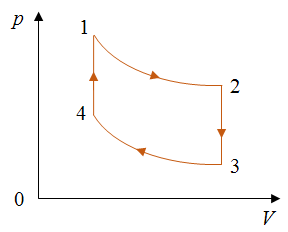
\includegraphics{images/cycle1.png}

		Чтобы понять, почему тепловые двигатели вообще могут совершать работу, достаточно посчитать, что

		\begin{equation*}
			A_{\text{газа}} = \int P S \d x = \int P \d V,
		\end{equation*}

		что соответствует площади фигуры внутри кривой на графике P-V.

		Простейшая модель теплового двигателя выглядит следующим образом. Есть \textbf{рабочее тело}, то есть газ, который будет совершать работу при своем расширении. Есть \textbf{нагреватель}, сообщающий теплоту рабочему телу. Однако этих двух элементов недостаточно, требуется также \textbf{холодильник}, которому рабочее тело отдает лишнюю теплоту, которую оно не смогло сконвертировать в работу. Под нагревателем и холодильником здесь понимаются не бытовые приборы, а любые тела, одно из которых горячее рабочего тела, а другое -- холоднее, например, топливо и атмосфера.

		Необходимость использования холодильника можно объяснить следующим образом. Будем следить, в каком состоянии на диаграмме P-V находится газ и отмечать адиабату, проходящую через текущую точку. При всех известных нам изопроцессах добавление теплоты приводит к переходу на более удаленную от начала координат адиабату. В верность этого факта для других процессов пока предлагается поверить. Тогда при добавлении теплоты газ перемещается с меньшей адиабаты на большую, соответственно, для перехода в обратную сторону требуется удаление тепла.

		Рабочее тело, таким образом, попеременно контактирует то с нагревателем, увеличивая при этом свою температуру, то с холодильником, уменьшая ее. При этом в перерывах между добавлением и удалением теплоты проводятся какие-то адиабатические процессы, потому что просто попеременного увеличения и уменьшения температуры, очевидно, недостаточно для совершения работы.

		Пусть $Q_{\text{н}}$ -- теплота, которую отдает нагреватель за один цикл, $Q_{\text{х}}$ -- теплота, передаваемая за цикл холодильнику за один цикл, $A = Q_{\text{н}} - Q_{\text{х}}$ -- работа за цикл. Тогда можно ввести КПД следующим образом:

		\namedequation{Коэффициент полезного действия}{\eta = \frac{A}{Q_{\text{н}}} = \frac{Q_{\text{н}} - Q_{\text{х}}}{Q_{\text{н}}}}

		В качестве примера рассматотрим один из простейших циклов теплового двигателя -- цикл Карно.

		\definition{Цикл Карно}{цикл теплового двигателя, состоящий из: изотермического расширения, адиабатного расширения, изотермического сжатия, адиабатного сжатия}

		\includesvg{images/carnot1}

		В начале цикла Карно (точка $A$ на диаграмме) рабочее тело нагрето до температуры нагревателя: $T = T_{\text{н}}$. В процессе $A \to B$ газ расширяется и совершает положительную работу, при этом сохраняя свою температуру за счет подведения к газу теплоты $Q_1$. В точке $B$ рабочее тело отсоединяется от нагревателя и далее ($B \to C$) расширяется адиабатически, уменьшая свою температуру $T$. Когда температура $T$ достигает $T_{\text{х}}$ в точке $C$, тело приводится в контакт с холодильником и сжимается с сохранением температуры за счет отведения от него теплоты $Q_2$, при этом тело совершает отрицательную работу. В точке $D$ холодильник отсоединяется от твердого тела, и газ дальше адиабатически сжимается до достижения состояния $A$, совершая отрицательную работу.

		При адиабатическом процессе $A \to B$ газ совершает работу, потому падает его температура, а это означает, что график адиабаты "круче" изотермы. Поэтому на графике P-V цикл Карно окружает фигуру, имеющую положительную площадь.

		Расчет работы, совершаемой тепловым двигателем, сводится к анализу связей между работой газа, внутренней энергией газа и подведенному количеству теплоты при изопроцессах. Из формул для изолиний получаем, что во время цикла Карно работа совершается следующим образом:

		\begin{align*}
			A_{A \to B} &= Q_{\text{н}} = \nu R T_{\text{н}} \ln \frac{V_1}{V_0}, \\
			A_{B \to C} &= \frac{i}{2} \nu R (T_{\text{н}} - T_{\text{х}}), \\
			A_{C \to D} &= -Q_{\text{х}} = -\nu R T_{\text{х}} \ln \frac{V_1}{V_0}, \\
			A_{D \to A} &= \frac{i}{2} \nu R (T_{\text{х}} - T_{\text{н}}).
		\end{align*}

		Таким образом, суммарная работа равна

		\begin{equation*}
			A = Q_{\text{н}} - Q_{\text{х}} = \nu R \left( T_{\text{н}} - T_{\text{х}} \right) \ln \frac{V_1}{V_0}.
		\end{equation*}

		КПД процесса:

		\begin{equation*}
			\eta = \frac{A}{Q_{\text{н}}} = \frac{\nu R \left( T_{\text{н}} - T_{\text{х}} \right) \ln \frac{V_1}{V_0}}{\nu R T_{\text{н}} \ln \frac{V_1}{V_0}} = \frac{T_{\text{н}} - T_{\text{х}}}{T_{\text{н}}}.
		\end{equation*}

		Оказывается, что совершенная за цикл работа зависит исключительно от разности температур нагревателя и холодильника. Исторически именно этот факт позволил определить линейную температурную шкалу. Измерения КПД, зависящего, как мы видим, от абсолютной температуры, позволили с большой точностью вычислить температуру абсолютного нуля.
	\end{section}


	\begin{section}{Второе начало термодинамики}
		В термодинамике мы часто сталкиваемся с \textbf{обратимыми процессами}. Это понятие означает, что некотором процесс можно провести в обратном направлении, при этом макроскопически все изменения будут противоположными по сравнению с прямым процессом. Под этим подразумевается в том числе и то, что работа, совершенная газом при прямом процессе, противоположна работе, совершенной им при обратном процессе.

		Многие из рассмотренных нами процессов являются обратимыми. Изобарное или изотермическое расширение можно обратить, проведя изобарное или изотермическое сжатие. Изохорный нагрев можно обратить, приведя тело в контакт с холодильником, которому будет отдана теплота. В некоторых ситуациях возможно провести обратимый адиабатический процесс.

		Обратимым является и цикл Карно -- при обращении он из тепловой машины превращается в тепловой насос, перегоняющий теплоту из более холодного тела к более теплому, потребляя при этом энергию.

		Изначально под обратимостью понималась возможность провести непрерывное изменение \textit{макропараметров} для возврата в исходное состояние. В такой интерпретации простейший пример необратимого процесса -- смешение газов разных температур. Когда молекулы разных газов перемешиваются, отделить их друг от друга макроскопическими средствами становится невозможно.

		Еще один пример -- приведение в контакт двух тел разной температуры и следующий из этого теплообмен. Для обращения такого процесса требуется передать энергию от более холодного тела к более теплому. В природе такого, как мы знаем, не происходит.

		Важный вопрос заключается в том, будут ли такие процессы необратимыми, если мы будем работать на уровне частиц, поскольку при этом ни один из известных нам законов сохранения не нарушается. В самом деле, для проведения обратного теплообмена между двумя газами можно создать некоторый инструмент -- \textbf{демон Максвелла}, -- который будет находиться на границе между резервуарами и пропускать в одну сторону только быстрые частицы, а в другую -- только медленные. Проблема заключается в том, что демон Максвелла сам является частью термодинамической системы, и на определение скорости частицы тратится некоторая энергия. Этот пример был взят за основу нового закона термодинамики:

		\namedlaw{Второе начало термодинамики}{Невозможен периодический процесс, единственным результатом которого будет передача теплоты от тела с меньшей температурой к телу с большей температурой.}

		Эквивалентное утвержедение -- невозможность периодического процесса, единственным результатом которого является полное преобразование внутренней энергии в механическую работу. В самом деле, если бы такая машина была возможна, мы бы могли конвертировать теплоту холодного тела в механическую работу и затем передавать ее горячему телу, что противоречит постулату.

		И наоборот: если бы можно было без притока энергии нагревать горячее тело от холодного, то можно было бы параллельно с этим процессом запустить тепловой двигатель с такой скоростью, чтобы температура холодного тела была постоянна. Такая система превращала бы теплоту в работу со стопроцентной эффективностью.

		Второе начало термодинамики имеет много последствий для тепловых двигателей -- области, где оно было открыто. Например, из него следует, что никакой тепловой двигатель не может быть более эффективным, чем обратимый двигатель. Если бы такое устройство существовало, его можно было бы запустить параллельно с обратимым двигателем, используемым в качестве теплового насоса, перегоняющего теплоту от холодильника к нагревателю и использующего в качестве источника энергии часть выходной работы устройства. Такая система переводила бы теплоту нагревателя в полезную работу со стопроцентной эффективностью. Следовательно:

		\begin{equation*}
			\eta_{\text{теплового двигателя}} \le \eta_{\text{обратимого теплового двигателя}}.
		\end{equation*}

		Можно пойти дальше, использовав в системе выше два обратимых двигателя. Если один из двигателей имеет больший КПД, чем другой, то мы приходим к аналогичному противоречию. Это означает, что КПД всех обратимых двигателей равны. Поскольку эффективность цикла Карно нам известна, мы получаем:

		\begin{equation*}
			\eta_{\text{обратимого теплового двигателя}} = \frac{T_{\text{н}} - T_{\text{х}}}{T_{\text{н}}}.
		\end{equation*}

		Отсюда также следует, что все обратимые двигатели эквивалентны в том смысле, что работа, совершаемая двигателем при данной теплоте нагревателя, не зависит от выбора двигателя и, следовательно, равенство

		\begin{equation*}
			\frac{Q_{\text{н}}}{T_{\text{н}}} = \frac{Q_{\text{х}}}{T_{\text{х}}}
		\end{equation*}

		выполняется не только для цикла Карно, но и для всех обратимых двигателей. Это можно интерпретировать так, что величина $\frac{Q}{T}$ в некотором смысле сохраняется в обратимых двигателях, хотя под $Q$ и $T$ понимаются несколько разные объекты в левой и правой части уравнения.

		Но важно понимать, что это равенство вытекает не столько из свойств цикла Карно, сколько из общих соображений.

		Выберем некоторую стандартную температуру $T_s$, равную единице температуры (абсолютной). Тогда любой обратимый тепловой двигатель можно заменить на систему из двух двигателей, один из которых перегоняет теплоту нагревателя в некоторый стандартный резервуар температуры $T_s$, а второй -- теплоту резервуара в теплоту холодильника, причем процессы сбалансированы так, что в среднем теплота стандратному резервуару не передается.

		Теплота, получаемая от нагревателя первым двигателем из этой системы, во-первых, зависит от температуры нагревателя, и во-вторых, пропорциональна теплоте, отданной стандартному резервуару:

		\begin{equation*}
			Q_1 = Q_s f(T_1),
		\end{equation*}

		где под $f$ понимается некоторая универсальная возрастающая функция от температуры.

		Аналогично для второго двигателя из системы:

		\begin{equation*}
			Q_2 = Q_s f(T_2).
		\end{equation*}

		Обратите внимание, что при этом выводе мы не пользовались определением температуры как меры внутренней энергии и какими либо вытекающими из этого фактами. Нам хватило лишь второго начала термодинамики и постулата о существовании температуры.

		Из свойств цикла Карно мы понимаем, что на самом деле $f$ линейна. Этот факт позволяет нам \textit{переопределить} температуру таким образом, что $f(T)$ пропорционально $T$, отвязав температуру от плохо поддающейся измерении внутренней энергии и привязав ее к эффективности обратимого двигателя.

		В такой интерпретации на передний план выходит величина $\frac{Q}{T}$. Мы уже знаем, что в цикле Карно она в некотором смысле сохраняется. Формально:

		\begin{equation*}
			\oint \frac{\delta Q}{T} = 0.
		\end{equation*}

		Это равенство можно вывести чисто математически из уравнения идеального газа:

		\begin{equation*}
			\frac{\delta Q}{T} = \frac{\d U + P \d V}{T} = \frac{i}{2} \nu R \frac{\d T}{T} + \nu R \frac{\d V}{V} = \frac{i}{2} \nu R \d \left( \ln TV^{\gamma - 1} \right).
		\end{equation*}

		Отсюда следует, что с величиной $\frac{\delta Q}{T}$ можно ассоциировать функцию состояния, несмотря на то, что $\delta Q$ является функцией процесса. То, что в уравнении появляется знакомое нам из адиабатического процесса выражение $TV^{\gamma - 1}$ -- ничуть не удивительно, ведь для адиабаты как раз $\delta Q = 0$.

		Величина, дифференциалом которой является $\frac{\delta Q}{T}$, называется \textbf{энтропией} и обозначается $S$. Мы уже показали, что для идеального газа с точностью до константы:

		\begin{equation*}
			S = \frac{i}{2} \nu R \ln T V^{\gamma - 1}.
		\end{equation*}

		Однако энтропия несет важный физический смысл, который такое чисто математическое объяснение несколько скрывает. Изменение энтропии в обратимом процессе численно равно теплоте, которая была бы при этом получена резервуаром единичной температуры.

		Энтропия является функцией состояния не только для идеальных газов, но и для любых систем. В самом деле, проведем следующий мысленный эксперимент. Рассмотрим систему, которая некоторым обратимым образом переводится из состояния $1$ в состояние $2$. Подготовим много резервуаров разных температур и в те моменты, когда система хочет отдать или получить теплоту, будем приводить ее в контакт с резервуаром, имеющим ту же температуру, что и система. Этим мы добиваемся отсутствия необратимого контакта тел разных температур. По окончании процесса в каждом резервуаре накопится некоторый избыток (возможно, отрицательный) теплоты $\delta Q_i$. Переведем все эти избытки в один резервуар при единичной температуре циклом Карно. Тогда для этого резервуара:

		\begin{equation*}
			\frac{\delta Q_s}{T_s} = \sum_i \frac{\delta Q_i}{T_i} = \delta S,
		\end{equation*}

		причем правая часть уравнения равна изменению энтропии за процесс.

		Предположим, что возможно провеси процесс некоторым другим обратимым путем, при котором изменение энтропии будет иное. В таком случае, проведя этот процесс в обратном направлении и опять перегнав избыток теплоты в стандартный резервуар, мы получим аналогичным образом

		\begin{equation*}
			\frac{\delta Q_s'}{T_s} = \delta S'.
		\end{equation*}

		Но тогда суммарно

		\begin{equation*}
			\frac{\delta Q_s' - \delta Q_s}{T_s} = \delta S - \delta S' \ne 0,
		\end{equation*}

		то есть существует обратимый процесс, единственным результатом которого является перевод теплоты в механическую работу или наоборот, что противоречит второму началу. Следовательно, изменение энтропии между состояниями не зависит от того, каким путем произошел переход, если только он обратим, что позволяет говорить об энтропии как о важнейшей функции состояния, наряду с температурой.

		Выражение

		\begin{equation*}
			\oint \frac{\delta Q}{T} = 0
		\end{equation*}

		не является законом сохранения в полном смысле этого слова, поскольку во время цикла энтропия рабочего тела не постоянна. Правильнее рассматривать не энтропию двигателя, а энтропию замкнутой системы, включающую в себя энтропию двигателя, нагревателя и холодильника:

		\begin{equation*}
			S = S_{\text{машины}} + S_{\text{н}} + S_{\text{х}}.
		\end{equation*}

		Элементарные изменения энтропии замкнутой системы происходят при передаче теплоты между ее частями. При передачи теплоты $\delta Q > 0$ от тела с температурой $T_1$ к телу с температурой $T_2$ энтропия системы меняется на

		\begin{equation*}
			\d S = \frac{\delta Q}{T_2} - \frac{\delta Q}{T_1}.
		\end{equation*}

		Второй закон термодинамики требует $T_1 \ge T_2$, отсюда

		\begin{equation*}
			\d S \ge 0,
		\end{equation*}

		причем равенство достигается при изотермическом теплообмене. Отсюда очевидно, что случай $\d S = 0 \iff T_1 = T_2$ соответствует обратимой передаче тепла, а $\d S > 0$ -- необратимой. Это позволяет ввести второе начало термодинамики математически:

		\namedlaw{Второе начало термодинамики (принцип возрастания энтропии)}{В замкнутой термодинамической системе энтропия неизменно возрастает: $\d S > 0$.}

		Строгость неравенство обусловлена тем, что провести изотермическую передачу теплоты на практике невозможно, поскольку для этого процесс требуется проводить с бесконечно малой скоростью.

		Во избежании путаницы лишний раз уточним, что изменение энтропии равно

		\begin{equation*}
			\Delta S = \int \frac{\delta Q}{T}
		\end{equation*}

		только для обратимых процессов; в необратимых процессах 

		\begin{equation*}
			\Delta S > \int \frac{\delta Q}{T},
		\end{equation*}

		что следует из второго закона термодинамики.

		Легко показать, что в циклических процессах помимо

		\begin{equation*}
			\oint \frac{\delta Q}{T} \ge 0
		\end{equation*}

		выполняется также \textbf{теорема Клаузиуса}:

		\begin{equation*}
			\oint \frac{\delta Q}{T_{\text{окр}}} \le 0,
		\end{equation*}

		где $T_{\text{окр}}$ есть температура резервуара, с которым происходит обмен теплотой.
	\end{section}
\end{document}
